%%%%%%%%%%%%%%%%%%%%%%%%%%%%%%%%%%%%%%%%%
% University/School Laboratory Report
% LaTeX Template
% Version 3.1 (25/3/14)
%
% This template has been downloaded from:
% http://www.LaTeXTemplates.com
%
% Original author:
% Linux and Unix Users Group at Virginia Tech Wiki 
% (https://vtluug.org/wiki/Example_LaTeX_chem_lab_report)
%
% License:
% CC BY-NC-SA 3.0 (http://creativecommons.org/licenses/by-nc-sa/3.0/)
%
%%%%%%%%%%%%%%%%%%%%%%%%%%%%%%%%%%%%%%%%%

%----------------------------------------------------------------------------------------
%	PACKAGES AND DOCUMENT CONFIGURATIONS
%----------------------------------------------------------------------------------------

\documentclass[twocolumn]{article}
% \documentclass{llncs}
% \usepackage{makeidx}


\usepackage[utf8]{inputenc}
\usepackage{graphicx} % Required for the inclusion of images
%\usepackage{natbib} % Required to change bibliography style to APA
\usepackage{amsmath} % Required for some math elements 
\usepackage{glossaries}
\usepackage[toc,page]{appendix}
\usepackage[autostyle=true]{csquotes}
\usepackage{hyperref}
\usepackage{amssymb}
\usepackage{caption} 
\usepackage{hhline}
\usepackage{float}
\usepackage{listings}
\usepackage{graphicx}
\usepackage{subcaption}

\setlength\parindent{0pt} % Removes all indentation from paragraphs

%\usepackage{times} % Uncomment to use the Times New Roman font

%----------------------------------------------------------------------------------------
%	DOCUMENT INFORMATION
%----------------------------------------------------------------------------------------

\title{The Art of Iterating:\\Update-Strategies in Agent-Based Simulations} % Title
 
\author{Jonathan \textsc{Thaler}} % Author name

\date{\today} % Date for the report

\begin{document}
%
\maketitle % Insert the title, author and date

% If you wish to include an abstract, uncomment the lines below
\begin{abstract}
When developing a model for an Agent-Based Simulation (ABS) it is of very importance to select the update-strategy which reflects the semantics of the model to produce the correct results. This awareness, we claim, is still lacking in the field of ABS. In this paper we present a novel terminology by systematic treatment of all general properties of ABS and deriving the general update-strategies. This will allow implementers and researchers in this field to use a general terminology thus removing ambiguities when discussing ABS and their models. Further we present a novel investigation into the suitability of three very different programming languages Java, Haskell and Scala with Actors to implement ABS in generality by implementing each of the update-strategies we derived.
\end{abstract}

\subsection*{Keywords}
Agent-Based Simulation, Parallelism, Concurrency, Haskell, Actors, Prisoners Dilemma, Heroes and Cowards

\section{Introduction}
There exists a large number of simulation packages which allow the convenient creation of System Dynamics simulations by straight-forward visual diagram creation. One simply creates stocks and flows, connects them, specifies the flow-rates and initial parameters and then runs the model. An example for such a visual diagram creation in the simulation package AnyLogic can be seen in Figure \ref{fig:sir_stockflow_diagram}.

\begin{figure}
	\centering
	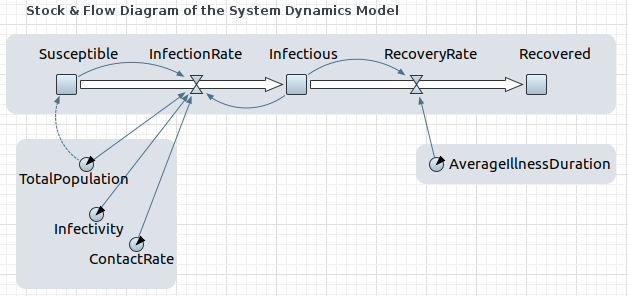
\includegraphics[width=.5\textwidth, angle=0]{./fig/SIR_SD_STOCKFLOW_DIAGRAMM.png}
	\caption{Visual System Dynamics Diagram of the SIR model in AnyLogic Personal Learning Edition 8.3.1.}
	\label{fig:sir_stockflow_diagram}
\end{figure}

Still, implementing System Dynamics directly in code is not as straight forward and involves numerical integration which can be quite tricky to get right. Thus, the aim of this paper is to look into how System Dynamics models can be implemented in code correctly without the use of a simulation package. We use the well known SIR model \cite{kermack_contribution_1927} from epidemiology to demonstrate our approach.

Our language of choice is Haskell because it emphasises a declarative programming style in which one describes \textit{what} instead of \textit{how} to compute. Further it allows to rule out interference with non-deterministic influences or side-effects already at compile-time. This is of fundamental importance for System Dynamics because it behaves completely deterministic and involves no stochastics or non-determinism whatsoever. Also, we make use of Functional Reactive Programming which allows to express continuous-time systems in a functional way. 

We show that by this approach we can arrive at correct-by-construction implementations of System Dynamic models. This means that the correctness of the code is obvious because we have closed the gap between the model specification and its implementation. Thus, the contribution of the paper is the demonstration of how to implement correct-by-construction System Dynamics simulations using Haskell and Functional Reactive Programming.

\section{Related Research}
Already noted in the Introduction, \cite{huberman_evolutionary_1993} where the first to discuss the differences update-strategies can make and introduced the terms of synchronous and asynchronous updates. They define to be synchronous as agents being updated in unison and asynchronous where one agent is updated and the others are held constant.

\medskip

\cite{a_framework_2008} give an approach for ABS on GPUs which is a very different approach to updating and iterating agents in ABS. They discuss execution order at length, highlight the problem of inducing a specific execution-order in a model which is problematic for parallel execution and give solutions how to circumvent these shortcomings. Although we haven't mapped our ideas to GPUs we explicitly include an approach for data-parallelism which, we hypothesize, can be utilized to roughly map their approach onto our terminology. 
	
\medskip
	
\cite{botta_time_2010} sketch a minimal ABS implementation in Haskell which is very similar in the basic structure of ours. This proves that our approach seems to be a very natural one to apply to Haskell. Their focus is primarily on economic simulations and instead of iterating a simulation with a global time, their focus is on how to synchronize agents which have internal, local transition times. Although their work uses Haskell as well, our focus is very different from theirs and approaches ABS in a more general and comprehensive way.

\medskip

\cite{dawson_opening_2014} describe basic inner workings of ABS environments and compare their implementation in C++ to the existing ABS environment AnyLogic which is programmed in Java. They explicitly mention asynchronous and synchronous time-models and compare them in theory but unfortunately couldn't report the results of asynchronous updates due to limited space. They interpret asynchronous time-models to be the ones in which an agent acts at random time intervals and synchronous time-models where agents are updated all in same time intervals.

\medskip

\cite{yuxuan_agent-based_2016} presents in his Master-Thesis a comprehensive discussion on how to implement an ABS for state-charts in Java and also mentions synchronous and asynchronous time-models. He identifies the asynchronous time-model to be one in which updates are triggered by the exchange of messages and the synchronous ones which trigger changes immediately without the indirection of messages.

\medskip

We observe that there seems to be a variety of meanings attributed to the terminology of asynchronous and synchronous updates but the very semantic and technical details are unclear and not described very precisely. In the next section we will address this issue by presenting the basic background and propose properties for a new terminology from which we can derive common update-strategies.

\chapter{Background}
\label{ch:background}

\section{Related research and literature}
\label{sec:literature}

The amount of research on using pure functional programming with Haskell in the field of ABS has been moderate so far. Most of the papers are related to the field of Multi Agent Systems (MAS) and look into how agents can be specified using the belief-desire-intention paradigm \cite{de_jong_suitability_2014,sulzmann_specifying_2007,jankovic_functional_2007}.

A multi-method simulation library in Haskell called \textit{Aivika 3} is described in the technical report \cite{sorokin_aivika_2015}. It supports implementing Discrete Event Simulations (DES), System Dynamics and comes with basic features for event-driven ABS which is realised using DES under the hood. Further it provides functionality for adding GPSS to models and supports parallel and distributed simulations. It runs within the IO effect type for realising parallel and distributed simulation but also discusses generalising their approach to avoid running in IO.

In his master thesis \cite{bezirgiannis_improving_2013} the author investigates Haskells' parallel and concurrency features to implement (amongst others) \textit{HLogo}, a Haskell clone of the NetLogo \cite{wilensky_introduction_2015} simulation package, focusing on using STM for a limited form of agent-interactions. \textit{HLogo} is basically a re-implementation of NetLogos API in Haskell where agents run within the IO context and thus can also make use of STM functionality. The benchmarks show that this approach does indeed result in a speed-up especially under larger agent-populations. The authors' thesis is one of the first on ABS using Haskell. Despite the concurrency and parallel aspect, this thesis approach is rather different: it avoids IO within the agents under all costs and explore the use of STM more on a conceptual level rather than implementing an ABS library to compare our case-studies with lock-based and imperative implementations.

There exists some research \cite{di_stefano_using_2005, varela_modelling_2004, sher_agent-based_2013} using the functional programming language Erlang \cite{armstrong_erlang_2010} to implement concurrent ABS. The language is inspired by the actor model \cite{agha_actors:_1986} and was created in 1986 by Joe Armstrong for Eriksson for developing distributed high reliability software in telecommunications. The actor model can be seen as quite influential to the development of the concept of agents in ABS, which borrowed it from Multi Agent Systems \cite{wooldridge_introduction_2009}. It emphasises message-passing concurrency with share-nothing semantics (no shared state between agents), which maps nicely to functional programming concepts. The mentioned papers investigate how the actor model can be used to close the conceptual gap between agent-specifications, which focus on message-passing and their implementation. Further they show that using this kind of concurrency allows to overcome some problems of low level concurrent programming as well.
Also \cite{bezirgiannis_improving_2013} ported NetLogos API to Erlang mapping agents to concurrently running processes, which interact with each other by message-passing. With some restrictions on the agent-interactions this model worked, which shows that using concurrent message-passing for parallel ABS is at least \textit{conceptually} feasible. Despite the natural mapping of ABS concepts to such an actor language, it leads to simulations, which despite same initial starting conditions, might result in different dynamics each time due to concurrency.

The work \cite{lysenko_framework_2008} discusses a framework, which allows to map Agent-Based Simulations to Graphics Processing Units (GPU). Amongst others they use the SugarScape model \cite{epstein_growing_1996} and scale it up to millions of agents on very large environment grids. They reported an impressive speed-up of a factor of 9,000. Although their work is conceptually very different this thesis draws inspiration from their work in terms of performance measurement and comparison to the Sugarscape model.

% THIS IS MY OWN REASEARCH, DON'T CITE IT HERE
%In \cite{thaler_pure_2019} the authors showed how to implement a spatial SIR model in pure Haskell using Functional Reactive Programming \cite{hudak_arrows_2003}. They report quite low performance but mention that STM may be a way to considerably speed up the simulation. We follow their approach in implementation technique, using Functional Reactive Programming and Monadic Stream Functions \cite{perez_functional_2016} (we don't go into implementation details as it is out of the scope of this paper) and use the spatial SIR model as the first case-study.

Using functional programming for DES was discussed in \cite{jankovic_functional_2007} where the authors explicitly mention the paradigm of Functional Reactive Programming (FRP) to be very suitable to DES.

A domain-specific language for developing functional reactive agent-based simulations was presented in \cite{schneider_towards_2012,vendrov_frabjous_2014}. This language called FRABJOUS is human readable and easily understandable by domain-experts. It is not directly implemented in FRP/Haskell but is compiled to Haskell code which they claim is also readable. This supports that FRP is a suitable approach to implement ABS in Haskell. Unfortunately, the authors do not discuss their mapping of ABS to FRP on a technical level, which would be of most interest to functional programmers.

Object-oriented programming and simulation have a long history together as the former one emereged out of Simula 67 \cite{dahl_birth_2002}, which was created for simulation purposes. Simula 67 already supported DES and was highly influential for today's object-oriented languages. Although the language was important and influential, in our research we look into different approaches, orthogonal to the existing object-oriented concepts.

Lustre is a formally defined, declarative and synchronous dataflow programming language for programming reactive systems \cite{halbwachs_synchronous_1991}. While it has solved some issues related to implementing ABS in Haskell, it still lacks a few important features necessary for ABS. There seems to be no way of implementing an environment in Lustre as it is done in Chapters \ref{ch:timedriven} and \ref{ch:eventdriven}. Also, the language seems not to come with stochastic functions, which are but the very building blocks of ABS. Finally, Lustre does only support static networks, which is clearly a drawback in ABS in general where agents can be created and terminated dynamically during simulation.

In \cite{botta_time_2010}, the authors discuss the problem of advancing time in message-driven agent-based socio-economic models. They formulate purely functional definitions for agents and their interactions through messages. Our architecture for synchronous agent-interaction as discussed in Chapter \ref{sec:eventdriven_implementation} was not directly inspired by their work but has some similarities: the use of messages and the problem of when to advance time in models which allows unrestricted synchronised agent interactions.

The authors of \cite{botta_functional_2011} are using functional programming as a specification for an agent-based model of exchange markets but leave the implementation for further research where they claim that it requires dependent types. This paper is the closest usage of dependent types in agent-based simulation we could find in the existing literature and to our best knowledge there exists no work on general concepts of implementing pure functional agent-based simulations with dependent types. %As a remedy to having no related work to build on, we looked into works which apply dependent types to solve real world problems from which we then can draw inspiration from.

In his talk \cite{sweeney_next_2006}, Tim Sweeney CTO of Epic Games discussed programming languages in the development of game engines and scripting of game logic. Although the fields of games and ABS seem to be very different, Gregory \cite{gregory_game_2018} defines computer-games as \textit{"[..] soft real-time interactive agent-based computer simulations"} (p. 9) and indeed, they have striking similarities: both are simulations which perform numerical computations and update objects in a loop either concurrently or sequential. In games these objects are called \textit{game-objects} and in ABS they are called \textit{agents} but they are conceptually the same thing.  Sweeney reports that reliability suffers from dynamic failure in languages like C++ e.g. random memory overwrites, memory leaks, accessing arrays out-of-bounds, dereferencing null pointers, integer overflow, accessing uninitialized variables. He reports that 50\% of all bugs in the Game Engine Middleware Unreal can be traced back to such problems and presents dependent types as a potential rescue to those problems. The two main points Sweeney made were that dependent types could solve most of the run-time failures and that parallelism is the future for performance improvement in games. He distinguishes between pure functional algorithms which can be parallelised easily in a pure functional language and updating game-objects concurrently using Software Transactional Memory (STM).

\section{Agent-Based Simulation}
\label{sec:method_abs}

%TODO RESTRUCTURING
%- classification according to \cite{macal_everything_2016}: macal paper \cite{macal_everything_2016}: very good survey/review paper on ABMS in General. fp can help with challenges h2, h4 and h5. also fp can help macals added transparency challenge, my thesis in general also adresses the knowledge challenge of macal "lack of abms educational...", note that we do NOT address ease-of-use as our approach is not easy to use. also the yampa approach can be seen as a hybrid approach of ABS/SD as posed as Research Challenge by macal. further STM might be one way of tackling large-scale ABS as identified as Research Challenge by macal. also this paper supports that ABS is a fundamentally new technique that offers the Potential to solve problems that are not robustly addressed by other methods
%\bigskip

This thesis understands ABS as a method and methodology to model and simulate a system, where the global behaviour may be unknown but the behaviour and interactions of the parts making up the system is known. Those parts, called agents, are modelled and simulated, out of which then the aggregate global behaviour of the whole system emerges. So, the central aspect of ABS is the concept of an agent, a metaphor for a pro-active unit, situated in an environment, able to spawn new agents and interacting with other agents in some neighbourhood by exchange of messages \cite{macal_everything_2016, odell_objects_2002, siebers_introduction_2008, wooldridge_introduction_2009}. Summarising, this thesis informally assumes the following about agents:

\begin{itemize}
	\item They are uniquely addressable entities with an internal state over which they have full, exclusive control.
	\item They are pro active, which means they can initiate actions on their own, for example change their internal state, send messages, create new agents, terminate themselves.
	\item They are situated in an environment and can interact with it.
	\item They can interact with other agents situated in the same environment by means of messaging.
\end{itemize} 

Epstein \cite{epstein_generative_2012} identifies ABS to be especially applicable for analysing \textit{"spatially distributed systems of heterogeneous autonomous actors with bounded information and computing capacity"}. Technically, ABS exhibits the following properties:

\begin{itemize}
	\item Linearity and non-linearity - actions of agents can lead to non-linear behaviour of the system.
	\item Time - agents act over time, which is also the source of their pro-activity.
	\item State - agents encapsulate state, which can be accessed and changed during the simulation.
	\item Feedback loop - because agents act continuously and their actions influence each other and themselves in the future of subsequent time steps, feedback loops permeate every ABS. 
	\item Heterogeneity - agents can have properties (age, height, sex,...) where the actual values can vary arbitrarily between individuals.
	\item Interactions - agents can be modelled after interactions with an environment and other agents.
	\item Spatiality and networks - agents can be situated within arbitrary environments, like spatial environments (discrete 2D, continuous 3D,...) or complex networks.
\end{itemize}

Note that there is no commonly agreed technical definition of ABS but the field draws inspiration from the closely related field of Multi-Agent Systems (MAS) \cite{weiss_multiagent_2013,wooldridge_introduction_2009}. It is important to understand that MAS and ABS are two different fields where in MAS the focus is much more on technical details, implementing a system of interacting intelligent agents within a highly complex environment with the focus primarily on solving AI problems.

\medskip

The field of ABS can be traced back to self-replicating von Neumann machines, cellular automata and Conway's Game of Life. The famous Schelling segregation model \cite{schelling_dynamic_1971} is regarded as a pioneering example. ABS as a discipline was first picked up by social simulation, which explores social norms, institutions, reputation, elections and economics. Axelrod \cite{axelrod_advancing_1997, axelrod_guide_2006} has called social simulation the third way of doing science, which he termed the \textit{generative} approach, which is in opposition to the classical inductive (finding patterns in empirical data) and deductive (proving theorems). Thus, the generative approach can be seen as a form of empirical research and is a natural environment for studying social and interdisciplinary phenomena as discussed more in depth in the work of Epstein \cite{epstein_chapter_2006, epstein_generative_2012}. He gives a fundamental introduction to agent-based social social simulation and makes the strong claim that \textit{"If you didn't grow it, you didn't explain its emergence"} \footnote{This can be seen as a fundamental constructivist approach to social science, which implies that the emergent properties are actually computable. When making connections from the simulation to reality, constructible emergence raises the question whether our existence is computable or not. When pushing this further, we can conjecture that the future of simulation will be simulated copies of our own existence, which potentially allows to simulate \textit{everything}. This idea is not new and an interesting treatment of it can be found in \cite{bostrom_are_2003, steinhart_theological_2010}.}. 
Epstein puts much emphasis on the claim that ABS is indeed a scientific instrument as hypotheses which are investigated are empirically falsifiable. If the simulation exhibits an emergent pattern, then the model is \textit{one} way of explaining it. On the other hand if it does not show the emergent pattern, then the hypothesis that the micro interactions amongst the agents generate the emergent pattern is falsified \footnote{This is fundamentally following Poppers theory of science \cite{popper_logic_2002}.} and we have not found an explanation \textit{yet}. So in summary, growing a phenomena is a necessary, but not sufficient condition for explanation \cite{epstein_chapter_2006}.

% NOTE: incorporate this only when there is enough time (and energy) to go through the 3 references cited here
%This raises a number of philosophical questions \cite{frigg_philosophy_2009}, \cite{grune-yanoff_philosophy_2010}, \cite{borrill_agent-based_2011}. Although we don't want to give an in-depth discussion of the questions raised, we want to have a quick look at them as this is a foundational research-proposal for a Doctor in \textit{Philosophy} (Ph.D.).
%TODO: read above papers and give short outline philosophical questions

The first large scale social ABS model which rose to some prominence was the \textit{Sugarscape} model developed by Epstein and Axtell in 1996 \cite{epstein_growing_1996}. Their aim was to \textit{grow} an artificial society by simulation and connect observations in their simulation to phenomenon of real-world societies. It was this simulation which strongly advertised object-oriented programming to implement ABS. Due to this influence and also due to the general popularity of the object-oriented paradigm which started to rise in the early-to-mid 90s, object-oriented programming has become the de-factor standard in implementing ABS . We can distinguish between three categories of how ABS is implemented today: % TODO: do we need citiations here to support our claims?
\begin{enumerate}
	\item Programming from scratch using object-oriented languages with Python, Java and C++ being the most popular ones.
	\item Programming using a 3rd party ABS library using object-oriented languages where RePast and DesmoJ, both in Java, are the most popular ones.
	\item Using a high-level ABS toolkit for non-programmers, which allow customisation through programming if necessary. By far the most popular one is NetLogo with an imperative programming approach followed by AnyLogic with an object-oriented Java approach.
\end{enumerate}

To get a better idea and deeper understanding of ABS, the next sections present two different, well-known agent-based models to give examples of two different types: the explanatory SIR model and the exploratory Sugarscape model. Both are used throughout the thesis as use cases for developing pure functional ABS implementation techniques, concepts and test beds for Software Transactional Memory and property-based testing.

% TODO: this is a nice blog: https://drewdevault.com/2018/07/09/Simple-correct-fast.html
% TODO: \cite{vipindeep_list_2005}
% TODO: software errors can be costly %https://raygun.com/blog/costly-software-errors-history/
% TODO: bugs per loc %https://www.mayerdan.com/ruby/2012/11/11/bugs-per-line-of-code-ratio

\section{Case Study I: SIR}
\label{sec:concurrent_sir}
Our first case study is the SIR model as introduced in Chapter \ref{sec:sir_model}. The aim of this case study is to investigate the potential speed up a concurrent \textit{STM} implementation gains over a sequential one under varying number of CPU cores and agents. The behaviour of the agents is quite simple and the interactions are happening indirectly through the environment, where reads from the environment outnumber the writes to it by far. Further, a comparison to a lock-based implementation with the \textit{IO} Monad is done to understand that \textit{STM} is also able to outperform traditional concurrency, \textit{in a pure functional ABS setting} while still retaining its greater static guarantees than \textit{IO} \footnote{The code of all three implementations is available at \url{https://github.com/thalerjonathan/phd/tree/master/public/stmabs/code/SIR}}.

\begin{enumerate}
	\item Sequential - this is the original implementation as discussed in Chapter \ref{sec:adding_env}, where the discrete 2D environment is shared amongst all agents as read-only data and the agents are executed sequentially within the main thread without any concurrency.
	\item STM - this is the same implementation as the \textit{Sequential} one but agents run now in the \textit{STM} Monad and have access to the discrete 2D environment through a transactional variable \textit{TVar}. This means that the agents now communicate indirectly by reads and writes through the \textit{TVar}.
	\item Lock-Based - this follows the \textit{STM} implementation, with the agents running in \textit{IO}. They share the discrete 2D environment using an \textit{IORef} and have access to an \textit{MVar} lock to synchronise access to it.
\end{enumerate}

Each experiment was run until $t = 100$ and stepped using $\Delta t = 0.1$. For each experiment we conducted 8 runs on our machine (see Table \ref{tab:machine_specs}) under no additional work-load and report the mean. %Further, we checked the visual outputs and the dynamics and they look qualitatively the same as the reference \textit{Sequential}. We could have used more rigour and properly validated the implementations against the formal specification using tests as we do in Chapter Property-based testing but we leave this for further res.
In the experiments we varied the number of agents (grid size) as well as the number of cores when running concurrently - the numbers are always indicated clearly.

\begin{table}
	\centering
	\begin{tabular}{ c || c }
		OS & Fedora 28, 64-bit \\ \hline
		RAM & 16 GByte \\ \hline
		CPU & Intel i5-4670K @ 3.4GHz \\ \hline
		HD & 250Gbyte SSD \\ \hline
		Haskell & GHC 8.2.2
	\end{tabular}
	
	\caption{Machine and Software specs for all experiments}
	\label{tab:machine_specs}
\end{table}

\subsection{Constant Grid Size, Varying Cores}
In this experiment we held the grid size constant to 51 x 51 (2,601 agents) and varied the cores. The results are reported in Table \ref{tab:constgrid_varyingcores}.

\begin{table}
	\centering
	\begin{tabular}{cc|c}
		\multicolumn{1}{ c||  }{\multirow{2}{*}{} } &
		\multicolumn{1}{ |c| }{Cores} & Duration      \\ \hline \hline 
		
		\multicolumn{1}{ c||  }{\multirow{1}{*}{Sequential} } &
		\multicolumn{1}{ |c| }{1} & 72.5      \\ \hline \hline 
		
		\multicolumn{1}{ c||  }{\multirow{4}{*}{Lock-Based} } &
		\multicolumn{1}{ |c| }{1} & 60.6       \\ \cline{2-3}
		\multicolumn{1}{ c||  }{}                       &
		\multicolumn{1}{ |c| }{2} & 42.8    \\ \cline{2-3}
		\multicolumn{1}{ c||  }{}                       &
		\multicolumn{1}{ |c| }{3} & 38.6    \\ \cline{2-3}
		\multicolumn{1}{ c||  }{}                       &
		\multicolumn{1}{ |c| }{4} & 41.6    \\ \hline \hline 
		
		\multicolumn{1}{ c||  }{\multirow{4}{*}{STM} } &
		\multicolumn{1}{ |c| }{1} & 53.2       \\ \cline{2-3}
		\multicolumn{1}{ c||  }{}                       &
		\multicolumn{1}{ |c| }{2} & 27.8    \\ \cline{2-3}
		\multicolumn{1}{ c||  }{}                       &
		\multicolumn{1}{ |c| }{3} & 21.8    \\ \cline{2-3}
		\multicolumn{1}{ c||  }{}                       &
		\multicolumn{1}{ |c| }{4} & \textbf{20.8}    \\ \hline \hline 
	\end{tabular}
  	
  	\caption{Experiments on 51x51 (2,601 agents) grid with varying number of cores. Timings in seconds (lower is better).}
	\label{tab:constgrid_varyingcores}
\end{table}

The \textit{STM} implementation running on 4 cores shows a speed up factor of 3.6 over \textit{Sequential}, which is a quite impressive number when considering that we can achieve at most a factor of 4 when running on 4 cores. It seems that \textit{STM} allow us to push the practical limit very close to the theoretical one, whereas the \textit{Lock-Based} approach just arrives at a factor of 1.74 on 4 cores.

Comparing the performance and scaling to multiple cores shows that the \textit{STM} implementation significantly outperforms the \textit{Lock-Based} one and scales better to multiple cores. The \textit{Lock-Based} implementation performs best with 3 cores and shows slightly worse performance on 4 cores as can be seen in Figure \ref{fig:core_duration_stm_io}. This is no surprise because the more cores are running at the same time, the more contention for the lock, thus the more likely synchronisation happening, resulting in higher potential for reduced performance. This is not an issue in \textit{STM} because no locks are taken in advance. 

\begin{figure}
	\centering
	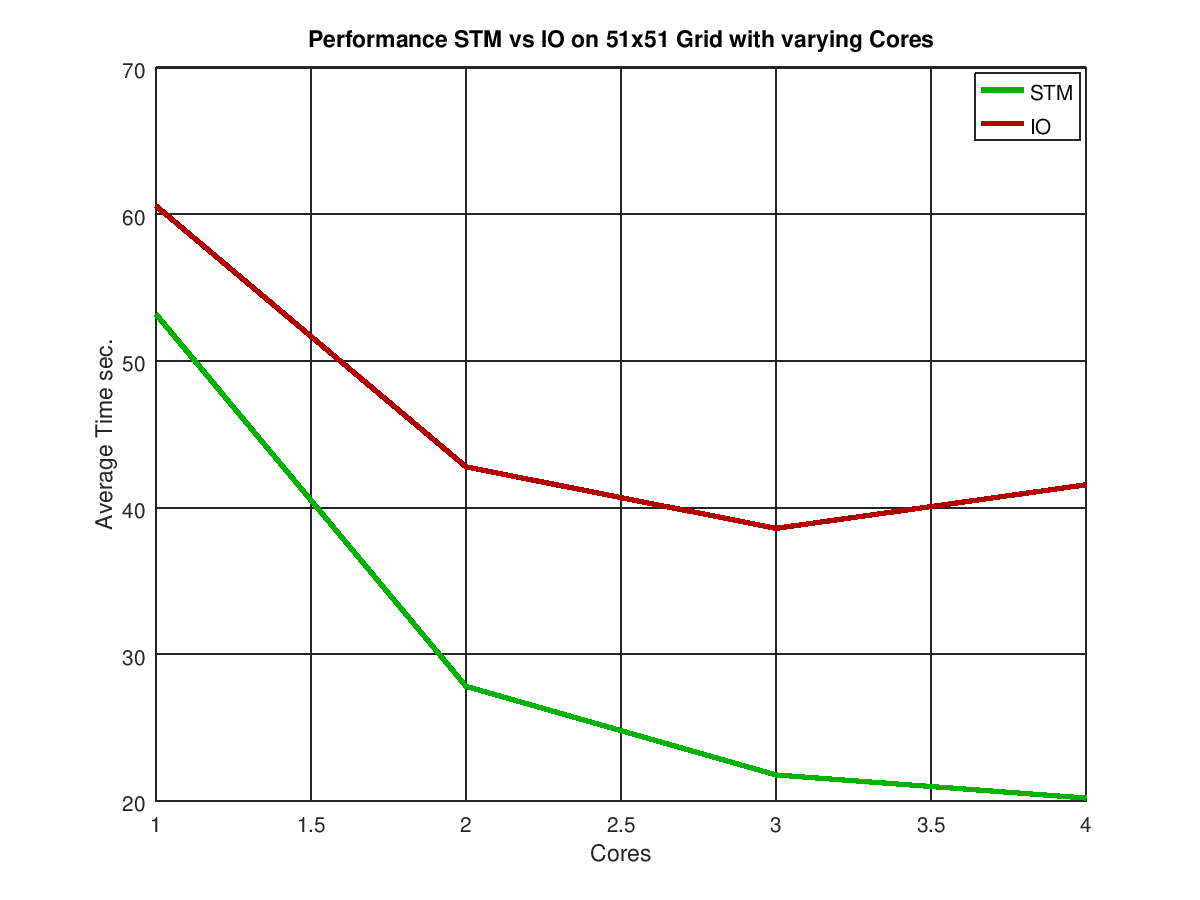
\includegraphics[width=0.8\textwidth, angle=0]{./fig/concurrentabs/sir/core_duration_stm_io.png}
	\caption{Comparison of performance and scaling on multiple cores of STM and Lock-Based. Note that the Lock-Based implementation seems to perform slightly worse on 4 than on 3 cores probably due to lock-contention.}
	\label{fig:core_duration_stm_io}
\end{figure}

\subsection{Varying Grid Size, Constant Cores}
In this experiment we varied the grid size and used always 4 cores. The results are reported in Table \ref{tab:varyinggrid_constcores} and plotted in Figure \ref{fig:varyinggrid_constcores}.

\begin{table}
	\centering
  	\begin{tabular}{ c || c | c | c }
        Grid-Size          & STM              & Lock-Based   & Ratio \\ \hline \hline 
   		51 x 51 (2,601)    & \textbf{20.2}    & 41.9         & 2.1 \\ \hline
   		101 x 101 (10,201) & \textbf{74.5}    & 170.5        & 2.3 \\ \hline
   		151 x 151 (22,801) & \textbf{168.5}   & 376.9        & 2.2 \\ \hline
   		201 x 201 (40,401) & \textbf{302.4}   & 672.0        & 2.2 \\ \hline
   		251 x 251 (63,001) & \textbf{495.7}   & 1,027.3      & 2.1 \\ \hline \hline
  	\end{tabular}

  	\caption{Performance on varying grid sizes. Timings in seconds (lower is better). Ratio compares STM to Lock-Based.}
	\label{tab:varyinggrid_constcores}
\end{table}

It is clear that the \textit{STM} implementation outperforms the \textit{Lock-Based} implementation by a substantial factor.

\begin{figure}
	\centering
	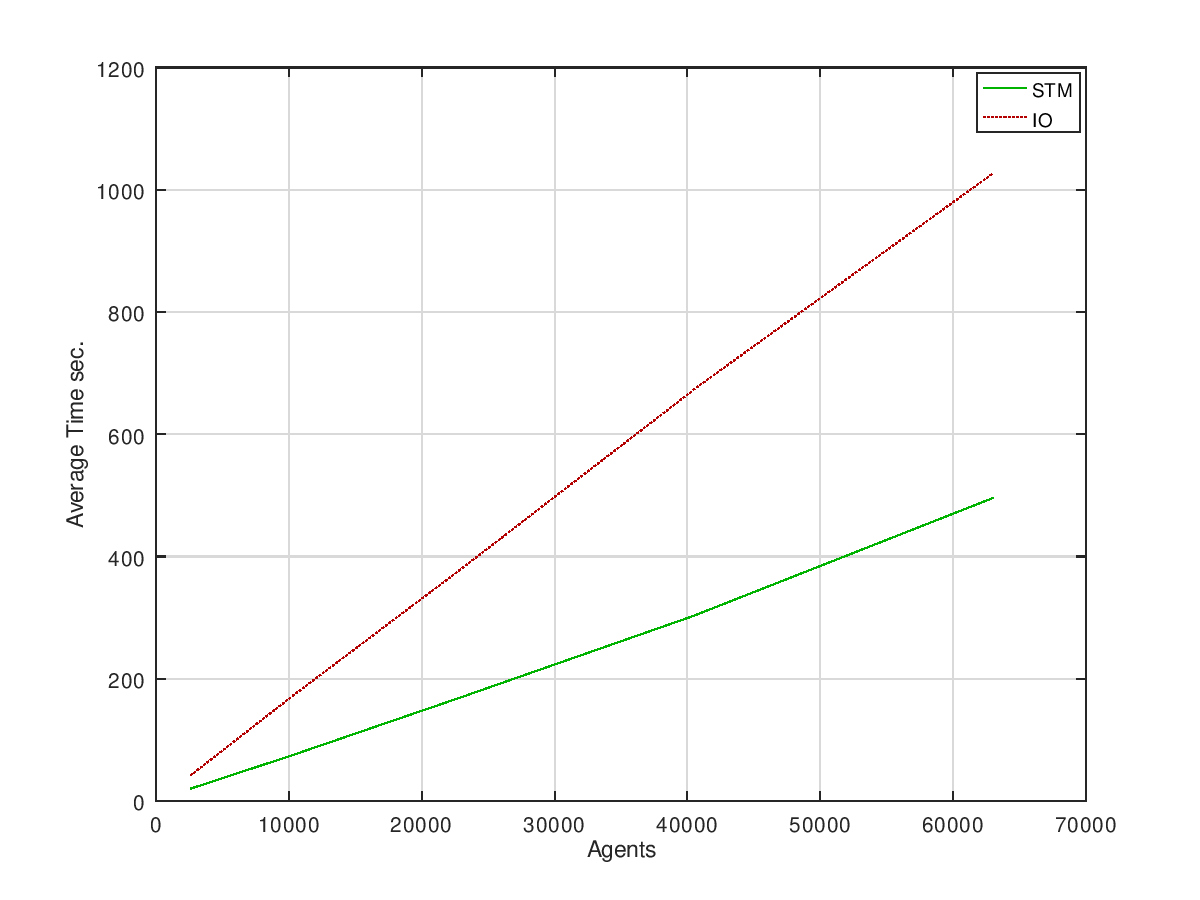
\includegraphics[width=1\textwidth, angle=0]{./fig/concurrentabs/sir/stm_io_varyinggrid_performance.png}
	\caption{Performance on varying grid sizes.}
	\label{fig:varyinggrid_constcores}
\end{figure}

\subsection{Retries}
Of very much interest when using STM is the retry-ratio, which obviously depends highly on the read-write patterns of the respective model. We used the \textit{stm-stats} library to record statistics of commits, retries and the ratio. The results are reported in Table \ref{tab:retries_stm}.

\begin{table}
	\centering
  	\begin{tabular}{ c || c | c | c }
        Grid-Size 		   & Commits    & Retries & Ratio \\ \hline \hline 
   		51 x 51 (2,601)    & 2,601,000  & 1306.5  & 0.0 \\ \hline
   		101 x 101 (10,201) & 10,201,000 & 3712.5  & 0.0 \\ \hline
   		151 x 151 (22,801) & 22,801,000 & 8189.5  & 0.0 \\ \hline
   		201 x 201 (40,401) & 40,401,000 & 13285.0 & 0.0 \\ \hline 
   		251 x 251 (63,001) & 63,001,000 & 21217.0 & 0.0 \\ \hline \hline
  	\end{tabular}
  	
  	\caption{Retry ratios on varying grid sizes on 4 cores.}
	\label{tab:retries_stm}
\end{table}

Independent of the number of agents we always have a retry-ratio of 0.0. This indicates that this model is \textit{very} well suited to STM, which is also directly reflected in the much better performance over the \textit{Lock-Based} implementation. Obviously this ratio stems from the fact that in our implementation we have \textit{very} few writes, which happen only in case when an agent changes from Susceptible to Infected or from Infected to Recovered. On the other hand, there are a very large number of reads due to indirect agent interaction. For \textit{STM} this is no problem because no lock is taken but the \textit{Lock-Based} approach is forced to conservatively take the lock to ensure mutual exclusive access to the critical section across all agents.

\subsection{Going Large-Scale}
To test how far we can scale up the number of cores in both the \textit{Lock-Based} and \textit{STM} cases, we ran two experiments, 51x51 and 251x251, on Amazon EC2 instances with a larger number of cores than our local machinery, starting with 16 and 32 to see if we are running into decreasing returns. The results are reported in Table \ref{tab:sir_varying_cores_amazon}.

\begin{table}
	\centering
  	\begin{tabular}{cc|c|c}
		\multicolumn{1}{ c||  }{\multirow{2}{*}{} } &
		\multicolumn{1}{ |c| }{Cores} & 51x51    & 251x251       \\ \hline \hline 
		
		\multicolumn{1}{ c||  }{\multirow{2}{*}{Lock-Based} } &
		\multicolumn{1}{ |c| }{16} & 72.5    & 1830.5       \\ \cline{2-4}
		\multicolumn{1}{ c||  }{}                       &
		\multicolumn{1}{ |c| }{32} & 73.1    & 1882.2      \\ \hline \hline 
		
		\multicolumn{1}{ c||  }{\multirow{2}{*}{STM} } &
		\multicolumn{1}{ |c| }{16} & \textbf{8.6}     & \textbf{237.0}       \\ \cline{2-4}
		\multicolumn{1}{ c||  }{}                       &
		\multicolumn{1}{ |c| }{32} & 12.0    & 248.7      \\ \hline \hline 
	\end{tabular}

  	\caption{Performance on varying cores on Amazon S2 Services. Timings in seconds (lower is better).}
	\label{tab:sir_varying_cores_amazon}
\end{table}

As expected, the \textit{Lock-Based} approach doesn't scale up to many cores because each additional core brings more contention to the lock, resulting in an even more decreased performance, even worse than the \textit{Sequential} implementation. This is particularly obvious in the 251x251 experiment because of the much larger number of concurrent agents. The \textit{STM} approach returns better performance on 16 cores but fails to scale further up to 32 where the performance drops below the one with 16 cores. In both STM cases we measured a retry-ratio of 0, thus we assume that with 32 cores we become limited by the overhead of STM transactions \cite{perfumo_limits_2008} because the workload of an STM action in our SIR implementation is quite small.

Compared to the \textit{Sequential} implementation, \textit{STM} reaches a speed up factor of 8.4 on 16 cores, which is still impressive but is much further away from the theoretical limit than in the case of only 4 cores -  a further indication that this model in particular and our approach in general does not scale up arbitrarily.

% NOTE: 0 retries in both cases means that the STM transactions themselves are becoming the bottleneck. this makes sens because the STM trasnactions in our SIR implementation are very small (especially recovered and infected agent) and could therefore really cause substantial overhead as pointed out by \cite{perfumo_limits_2008}
%16 cores 251x251: 0.0 retry-ratio
%32 cores 251x251: 0.0 retry ratio
%
%16 cores 51x51: 0.0 retry-ratio
%32 cores 51x51: 0.0 retry ratio

\subsection{Discussion}
The timing measurements speak a clear language: running in \textit{STM} and sharing state using a transactional variable \textit{TVar} is much more time-efficient than both the \textit{Sequential} and \textit{Lock-Based} approach. On 4 cores \textit{STM} achieves a speed up factor of 3.6, nearly reaching the theoretical limit.
Obviously both \textit{STM} and \textit{Lock-Based} sacrifices determinism: repeated runs might not lead to same dynamics despite same initial conditions. Still, by sticking to \textit{STM}, we get the guarantee that the source of this non-determinism is concurrency within the \textit{STM} monad but \textit{nothing else}. This we can not guarantee in the case of the \textit{Lock-Based} approach as all bets are off when running within \textit{IO}. The fact to have \textit{both} the better performance \textit{and} the stronger static guarantees in the \textit{STM} approach makes it \textit{very} compelling.

\section{Case Study II: Sugarscape}
\label{sec:sugarscape_concurrent}
The second case study is the Sugarscape model as introduced in Chapter \ref{sec:sugarscape}. In this case study we look into the potential performance improvement in a model with much more complex agent behaviour and dramatically increased writes on the shared environment.

We implemented the \textit{Carrying Capacity} (p. 30) section of Chapter II of the Sugarscape book \cite{epstein_growing_1996}. In each step agents search (move) to the cell with the most sugar they see within their vision, harvest all of it from the environment and consume sugar because of their metabolism. Sugar regrows in the environment over time. Only one agent can occupy a cell at a time. Agents don't age and cannot die from age. If agents run out of sugar due to their metabolism, they die from starvation and are removed from the simulation. The authors report that the initial number of agents quickly drops and stabilises around a level depending on the model parameters. This is in accordance with our results as we show in Chapter \ref{ch:property} and guarantees that we don't run out of agents. The model parameters are as follows:

\begin{itemize}
	\item Sugar Endowment: each agent has an initial sugar endowment randomly uniform distributed between 5 and 25 units;
	\item Sugar Metabolism: each agent has a sugar metabolism randomly uniform distributed between 1 and 5;
	\item Agent Vision: each agent has a vision randomly uniform distributed between 1 and 6, same for each of the 4 directions (N, W, S, E);
	\item Sugar Growback: sugar grows back by 1.0 unit per step until the maximum capacity of a cell is reached;
	\item Agent Number: initially 500 agents;
	\item Environment Size: 50 x 50 cells with toroid boundaries which wrap around in both x and y dimension.
\end{itemize}

Note that in this implementation (as in the full Chapter II of the book), no direct and no synchronous agent-interactions as we implemented them in Chapter \ref{sec:eventdriven_implementation} are happening. As in the SIR example, all agents interact with each other indirectly through the shared environment. This allows us to regard the implementation as a time-driven, parallel one wherein each step agents act conceptually at the same time.

We compare four different implementations \footnote{The code is freely available at \url{https://github.com/thalerjonathan/phd/tree/master/public/stmabs/code/SugarScape}}:

\begin{enumerate}
	\item Sequential - All agents are run after another (including the environment) and the environment is shared amongst the agents using a \textit{StateT} transformer.
	\item Lock-Based - All agents are run concurrently in the \textit{IO} monad and the environment is shared between the agents, using an \textit{IORef} with the access synchronised through an \textit{MVar} lock.
	\item STM TVar - All agents are run concurrently in the \textit{STM} monad and the environment is shared using a \textit{TVar} between the agents.
	\item STM TArray - All agents are run concurrently in the \textit{STM} monad and the environment is shared using a \textit{TArray} between the agents. 
\end{enumerate}

We follow \cite{lysenko_framework_2008} and measure the average number of steps per second of the simulation over 60 seconds. For each experiment we conducted 8 runs on our machine (see Table \ref{tab:machine_specs}) under no additional work-load and report the average. In the experiments we varied the number of cores when running concurrently - the numbers are always indicated clearly.

%\paragraph{Output} Note that we omit the graphical rendering in the functional approach because it is a serious bottleneck taking up substantial amount of the simulation time. Although visual output is often important in ABS, it is not what we are interested here thus we completely omit it and only output the number of agents in the simulation at each step piped into a file, thus omitting slow output to the console \footnote{Note that we need to produce \textit{some} output because of Haskells laziness - if we wouldn't output anything from the simulation then the expressions would actually never be fully evaluated thus resulting in high number of steps per second but which obviously don't really reflect the true computations done.}.

\paragraph{Ordering} The model specification requires to shuffle agents before every step (Footnote 12 on page 26 \cite{epstein_growing_1996}). In the \textit{Sequential} approach we do this explicitly but in the \textit{Lock-Based} and both \textit{STM} approaches we assume this to happen automatically due to race-conditions in concurrency, thus we arrive at an effectively shuffled processing of agents: we implicitly assume that the order of the agents is \textit{effectively} random in every step. The important difference between the two approaches is that in the \textit{Sequential} approach we have full control over this randomness but in the \textit{STM} not - also this means that repeated runs with the same initial conditions might lead to slightly different results. 
This decision leaves the execution order of the agents ultimately to Haskell's Runtime System and the underlying OS. We are aware that by doing this, we make assumptions that the threads run uniformly distributed (fair) but such assumptions should not be made in concurrent programming. As a result we can expect this fact to produces non-uniform distributions of agent runs but we assumed that for this model this does not has a significance influence - in case of doubt, we could resort to shuffling the agents before running them in every step. We agree that this very problem would deserve in-depth research on its own, where also the influence of non-deterministic ordering on the correctness and results of ABS has to be analysed. This is not the main interest of this section though and we leave it for further research as it is completely beyond the focus of this thesis.

%Note that in the concurrent implementations we have two options for running the environment: either asynchronously as a concurrent agent at the same time with the population agents or synchronously after all agents have run. We must be careful though as running the environment as a concurrent agent can be seen as conceptually wrong because the time when the regrowth of the sugar happens is now completely random. In this case it could happen that sugar regrows in the very first transaction or in the very last, different in each step, which can be seen as a violation of the model specifications. Thus we do not run the environment concurrently with the agents but synchronously after all agents have run.

\subsection{Constant Agent Size}
In a first approach we compare the performance of all implementations on varying numbers of cores. The results are reported in Table \ref{tab:varying_cores} and plotted in Figure \ref{fig:varying_cores}. 

\begin{table}
	\centering
	\begin{tabular}{cc|c|c}
		\multicolumn{1}{ c||  }{\multirow{2}{*}{} } &
		\multicolumn{1}{ |c| }{Cores} & Steps & Retries      \\ \hline \hline 
		
		\multicolumn{1}{ c||  }{\multirow{1}{*}{Sequential} } &
		\multicolumn{1}{ |c| }{1} & 39.4 & N/A     \\ \hline \hline 
		
		\multicolumn{1}{ c||  }{\multirow{4}{*}{Lock-Based} } &
		\multicolumn{1}{ |c| }{1} & 43.0 & N/A       \\ \cline{2-4}
		\multicolumn{1}{ c||  }{}                       &
		\multicolumn{1}{ |c| }{2} & 51.8 & N/A   \\ \cline{2-4}
		\multicolumn{1}{ c||  }{}                       &
		\multicolumn{1}{ |c| }{3} & 57.4 & N/A   \\ \cline{2-4}
		\multicolumn{1}{ c||  }{}                       &
		\multicolumn{1}{ |c| }{4} & 58.1 & N/A   \\ \hline \hline 
		
		\multicolumn{1}{ c||  }{\multirow{4}{*}{STM \textit{TVar}} } &
		\multicolumn{1}{ |c| }{1} & \textbf{47.3} & 0.0       \\ \cline{2-4}
		\multicolumn{1}{ c||  }{}                       &
		\multicolumn{1}{ |c| }{2} & 53.5 & 1.1    \\ \cline{2-4}
		\multicolumn{1}{ c||  }{}                       &
		\multicolumn{1}{ |c| }{3} & 57.1 & 2.2    \\ \cline{2-4}
		\multicolumn{1}{ c||  }{}                       &
		\multicolumn{1}{ |c| }{4} & 53.0 & 3.2   \\ \hline \hline 
		
		\multicolumn{1}{ c||  }{\multirow{4}{*}{STM \textit{TArray}} } &
		\multicolumn{1}{ |c| }{1} & 45.4 & 0.0       \\ \cline{2-4}
		\multicolumn{1}{ c||  }{}                       &
		\multicolumn{1}{ |c| }{2} & \textbf{65.3} & 0.02   \\ \cline{2-4}
		\multicolumn{1}{ c||  }{}                       &
		\multicolumn{1}{ |c| }{3} & \textbf{75.7} & 0.04    \\ \cline{2-4}
		\multicolumn{1}{ c||  }{}                       &
		\multicolumn{1}{ |c| }{4} & \textbf{84.4} & 0.05   \\ \hline \hline 
	\end{tabular}  	
  	
  	\caption{Steps per second and retries on 50x50 grid with 500 initial agents on varying cores.}
	\label{tab:varying_cores}
\end{table}

\begin{figure}
	\centering
	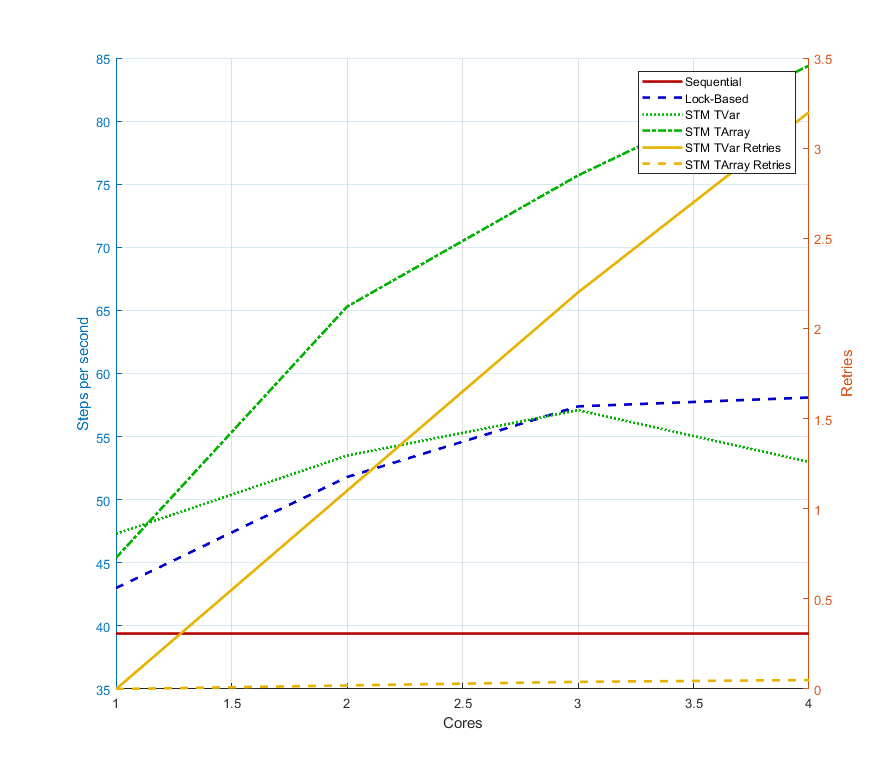
\includegraphics[width=0.7\textwidth, angle=0]{./fig/concurrentabs/sugarscape/varying_cores.png}
	\caption{Steps per second and retries on 50x50 grid and 500 initial agents on varying cores.}
	\label{fig:varying_cores}
\end{figure}

As expected, the \textit{Sequential} implementation is the slowest, followed by the \textit{Lock-Based} and \textit{TVar} approach whereas \textit{TArray} is the best performing one.

We clearly see that using a \textit{TVar} to share the environment is a very inefficient choice in this model: \textit{every} write to a cell leads to a retry independent whether the reading agent reads that changed cell or not, because the data-structure can not distinguish between individual cells. By using a \textit{TArray} we can avoid the situation where a write to a cell in a far distant location of the environment will lead to a retry of an agent which never even touched that cell. Also the \textit{TArray} seems to scale up by 10 steps per second for every core added. It will be interesting to see how far this could go with the Amazon experiment, as we seem not to hit a limit with 4 cores yet.

The inefficiency of \textit{TVar} is also reflected in the nearly similar performance of the \textit{Lock-Based} implementation which even outperforms it on 4 cores. This is due to very similar approaches because both operate on the whole environment instead of only the cells as \textit{TArray} does. This seems to be a bottleneck in \textit{TVar} reaching the best performance on 3 cores, which then drops on 4 cores due to an increasing retries ratio. The \textit{Lock-Based} approach seems to reduce its returns on increased number of cores hitting a limit at 4 cores as well.

\subsection{Scaling up Agents}
So far we kept the initial number of agents at 500, which due to the model specification, quickly drops and stabilises around 200 due to the carrying capacity of the environment as described in the book \cite{epstein_growing_1996} section \textit{Carrying Capacity} (p. 30).

We now want to measure the performance of our approaches under increased number of agents. For this we slightly change the implementation: always when an agent dies it spawns a new one which is inspired by the ageing and birthing feature of Chapter III in the book \cite{epstein_growing_1996}. This ensures that we keep the number of agents roughly constant (still fluctuates but doesn't drop to low levels) over the whole duration. This ensures a constant load of concurrent agents interacting with each other and demonstrates also the ability to terminate and create concurrent agents (threads) dynamically during the simulation.

Except for the \textit{Sequential} approach we ran all experiments with 4 cores (TVar with 3 as well). We looked into the performance of 500, 1,000, 1,500, 2,000 and 2,500 (maximum possible capacity of the 50x50 environment). The results are reported in Table \ref{tab:state_results_agentsscale_time} and plotted in Figure \ref{fig:state_results_agentsscale_time}.

\begin{table}
	\centering
  	\begin{tabular}{ c || c | c | c | c | c }
        Agents  & Sequential & Lock-Based & TVar (3 cores) & TVar (4 cores) & TArray  \\ \hline \hline 
    	    500     & 14.4       & 20.2		  &	20.1           & 18.5       	& \textbf{71.9}    \\ \hline
   		1,000   & 6.8        & 10.8 	      & 10.4           & 9.5         & \textbf{54.8}    \\ \hline
   		1,500   & 4.7        & 8.1 		  & 7.9            & 7.3			& \textbf{44.1}    \\ \hline
   		2,000   & 4.4        & 7.6 		  & 7.4            & 6.7    		& \textbf{37.0}    \\ \hline 
   		2,500   & 5.3        & 5.4 		  & 9.2            & 8.9			& \textbf{33.3}    \\ \hline \hline
   	\end{tabular}
  	
  	\caption{Steps per second on 50x50 grid with varying number of agents with 4 (and 3) cores except Sequential (1 core).}
	\label{tab:state_results_agentsscale_time}
\end{table}

\begin{figure}
	\centering
	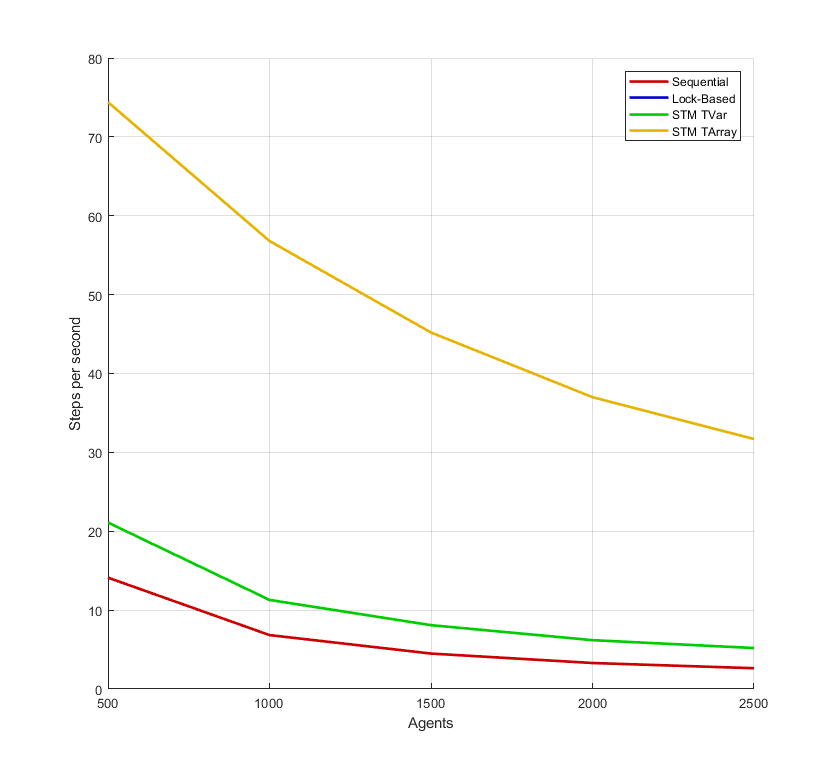
\includegraphics[width=1.0\textwidth, angle=0]{./fig/concurrentabs/sugarscape/varying_agents.png}
	\caption{Steps per second on 50x50 grid and varying number of agents with 4 (and 3) cores except Sequential (1 core).}
	\label{fig:state_results_agentsscale_time}
\end{figure}

As expected, the \textit{TArray} implementation outperforms all others substantially. Also as expected, the \textit{TVar} implementation on 3 cores is faster than on 4 cores as well when scaling up to more agents. The \textit{Lock-Based} approach performs about the same as the \textit{TVar} on 3 cores because of the very similar approaches: both access the \textit{whole} environment. Still the \textit{TVar} approach uses one core less to arrive at the same performance, thus strictly speaking outperforming the \textit{Lock-Based} implementation.

What seems to be very surprising is that in the \textit{Sequential} and \textit{TVar} cases the performance with 2,500 agents is \textit{better} than the one with 2,000 agents. The reason for this is that in the case of 2,500 agents, an agent can't move anywhere because all cells are already occupied. In this case the agent won't rank the cells in order of their pay-off (max sugar) to move to but just stays where it is. We hypothesize that due to Haskells laziness the agents actually never look at the content of the cells in this case but only the number which means that the cells themselves are never evaluated which further increases performance. This leads to the better performance in case of \textit{Sequential} and \textit{TVar} because both exploit laziness.
In the case of the \textit{Lock-Based} approach we still arrive at a lower performance because the limiting factor are the unconditional locks. In the case of the \textit{TArray} approach we also arrive at a lower performance because it seems that STM perform reads on the neighbouring cells which are not subject to lazy evaluation. In Haskell it is notoriously difficult to reason about efficiency (see Chapter \ref{ch:drawbacks} for a short discussion on drawbacks) and this behaviour of improved performance due to Haskells lazyness is no exception. We leave an in-depth investigation for further research as it is beyond the focus of this chapter.

We also measured the average retries both for \textit{TVar} and \textit{TArray} under 2,500 agents where the \textit{TArray} approach shows best scaling performance with 0.01 retries whereas \textit{TVar} averages at 3.28 retries. Again this can be attributed to the better transactional data-structure which reduces retry-ratio substantially to near-zero levels.

\subsection{Going Large-Scale}
To test how far we can scale up the number of cores in both the \textit{Lock-Based} and \textit{TArray} cases, we ran the two experiments (carrying capacity and rebirthing) on Amazon EC2 instances with increasing number of cores starting with 16 and 32 to see if we run into decreasing returns. The results are reported in Table \ref{tab:sug_varying_cores_amazon}.

\begin{table}
	\centering
%  	\begin{tabular}{ c || c | c | c }
%                   & Cores & Carrying Capacity & Rebirthing  \\ \hline \hline 
%    	Lock-Based & 16    & 53.9              & 4.4         \\ \hline
%    	Lock-Based & 32    & 44.2              & 3.6         \\ \hline \hline 
%   		
%   		STM TArray & 16    & \textbf{116.8} (0.23)      & \textbf{39.5} (0.08) \\ \hline
%   		STM TArray & 32    & 109.8 (0.41)      & 31.3 (0.18) \\ \hline \hline 
%   	\end{tabular}
  	
	\begin{tabular}{cc|c|c}
		\multicolumn{1}{ c||  }{\multirow{2}{*}{} } &
		\multicolumn{1}{ |c| }{Cores} & Carrying Capacity    & Rebirthing       \\ \hline \hline 
		
		\multicolumn{1}{ c||  }{\multirow{2}{*}{Lock-Based} } &
		\multicolumn{1}{ |c| }{16} & 53.9              & 4.4       \\ \cline{2-4}
		\multicolumn{1}{ c||  }{}                       &
		\multicolumn{1}{ |c| }{32} & 44.2              & 3.6      \\ \hline \hline 
		
		\multicolumn{1}{ c||  }{\multirow{2}{*}{STM TArray} } &
		\multicolumn{1}{ |c| }{16} & \textbf{116.8} (0.23)      & \textbf{39.5} (0.08)       \\ \cline{2-4}
		\multicolumn{1}{ c||  }{}                       &
		\multicolumn{1}{ |c| }{32} & \textbf{109.8} (0.41)      & \textbf{31.3} (0.18)      \\ \hline \hline 
	\end{tabular}  	
  	
  	\caption{Steps per second on varying cores on Amazon S2 Services.}
	\label{tab:sug_varying_cores_amazon}
\end{table}

As expected, the \textit{Lock-Based} approach doesn't scale up to many cores because each additional core brings more contention to the lock, resulting in even more decreased performance. This is particularly obvious in the rebirthing experiment because of the much larger number of concurrent agents. The \textit{TArray} approach returns better performance on 16 cores but fails to scale further up to 32 where the performance drops below the one with 16 cores. We indicated the retry-ratio in brackets and see that they roughly double from 16 to 32, which is the reason why performance drops as at this point. 

%the INCREASE in time can only happen due to more retries
%Carrying Capacity 16 core ~ 0.23 retry-ratio
%Carrying Capacity 32 core ~ 0.41 retry-ratio
%
%Rebirthing 16 core ~ 0.08 retry-ratio
%Rebirthing 32 core ~ 0.18 retry-ratio

\subsection{Comparison with other approaches}
The paper \cite{lysenko_framework_2008} reports a performance of 17 steps in RePast, 18 steps in MASON (both non-parallel) and 2,000 steps per second on a GPU on a 128x128 grid. Although our \textit{Sequential} implementation, which runs non-parallel as well, outperforms the RePast and MASON implementations of \cite{lysenko_framework_2008}, one must be very well aware that these results were generated in 2008, on current hardware of that time.

%When we run the SugarScape example of RePast with the same model parameters as ours on the same machine (see Table \ref{tab:machine_specs}) we arrive at roughly 450 steps per second - a factor of about 3.8 faster than even our STM \textit{TArray} implementation on 16 cores. This might seem quite shocking, even more so because RePast also performs visual output, rendering the SugarScape in every step. When scaling up the agents to 2,500 the RePast version arrives around roughly 95 steps per second which is still faster by a factor of 3 than our 4 core \textit{TArray} implementation. We attribute this substantial performance difference to the inherent performance difference of functional programming to imperative approaches as already outlined in the previous section. 

The very high performance on the GPU does not concern us here as it follows a very different approach than ours. We focus on speeding up implementations on the CPU as directly as possible without locking overhead. When following a GPU approach one needs to map the model to the GPU which is a delicate and non-trivial matter. With our approach we show that speed up with concurrency is very possible without the low-level locking details or the need to map to GPU. Also some features as bilateral trading between agents, where a pair of agents needs to come to a conclusion over multiple synchronous steps, is difficult to implement on a GPU whereas this is easily possible using STM.

Note that we kept the grid-size constant because we implemented the environment as a single agent which works sequentially on the cells to regrow the sugar. Obviously this doesn't really scale up on parallel hardware and experiments which we haven't included here due to lack of space, show that the performance goes down dramatically when we increase the environment to 128x128 with same number of agents which is the result of Amdahl's law where the environment becomes the limiting factor of the simulation. Depending on the underlying data-structure used for the environment we have two options to solve this problem. In the case of the \textit{Sequential} and \textit{TVar} implementation we build on an indexed array, which we can be updated in parallel using the existing data-parallel support in Haskell. In the case of the \textit{TArray} approach we have no option but to run the update of every cell within its own thread. We leave both for further research as it is out of scope of this paper.

\subsection{Discussion}
This case study showed clearly that besides being substantially faster than the \textit{Sequential} implementation, \textit{STM} is also able to perform considerably better than a \textit{Lock-Based} approach even in the case of a model with much higher complexity in agent behaviour and dramatically increased number of writes to the environment.
Further, this case study demonstrated that the selection of the right transactional data-structure is of fundamental importance when using \textit{STM}. Selecting the right transactional data-structure is very model-specific and can lead to dramatically different performance results.
In this case the \textit{TArray} performed best due to many writes but in the SIR case-study a \textit{TVar} showed good enough results due to the very low number of writes. When not carefully selecting the right transactional data-structure which supports fine-grained concurrency, a lock-based implementation might perform as well or even outperform the STM approach as can be seen when using the \textit{TVar}.
Although the \textit{TArray} is the better transactional data-structure overall, it might come with an overhead, performing worse on low number of cores than a \textit{TVar} approach but has the benefit of quickly scaling up to multiple cores. Depending on the transactional data-structure, scaling up to multiple cores hits a limit at some point. In the case of the \textit{TVar} the best performance is reached with 3 cores. With the \textit{TArray} we reached this limit around 16 cores.

Note that the comparison between the \textit{Lock-Based} approach and the \textit{STM TArray} implementation is a bit unfair due to a very different locking structure. A more suitable comparison would have been to use an indexed Array with a tuple of (MVar, IORef) in each cell to support fine-grained locking on cell-level. This would be a more just comparison to the \textit{STM Array} where fine-grained transactions happen on the cell-level. We hypothesize that \textit{STM} will still outperform the \textit{IO} approach but to a lesser degree - we leave the proof of this for further research.

%Unfortunately, for this model the performance is nowhere comparable to imperative approaches, which we attribute to the inherent performance difference of functional programming to imperative approaches. With the use of advanced language features we might arrive at much improved performance but we leave this for further research as we focus primarily on the comparison between lock-based and STM approaches.

%we can implement everything except synchronous direct agent-interactions atm: if agent-interaction is one-way e.g. paying back a loan then this is no problem. thus the following parts of the Sugarscape are not possible with our current STM approach: mating, trading and lending  because all 3 require direct agent-to-agent interaction over multiple steps. We leave the problem of developing such an algorithm / implementation for further research.

\section{Pure Functional Programming}
\label{sec:background_fp}
To be able to understand the challenges of pure functional ABS as well as the solutions and concepts developed in this thesis, in this section we give a short introduction to functional programming, with an overview of its concepts and advanced features. As it is obviously beyond the focus of a thesis to give a full treatment of such a complex topic, we refer to additional literature and references for further discussions where appropriate.

Functional programming is called \textit{functional} because it makes functions the main concept of programming, promoting them to first-class citizens. This means that functions can be assigned to variables, they can be passed as arguments to other functions and they can be constructed as return values from functions. The roots of functional programming lie in Lambda Calculus which was first described by Alonzo Church \cite{church_unsolvable_1936}. This is a fundamentally different approach to computing than imperative programming (including established object-orientation), the roots of which lie in the Turing Machine \cite{turing_computable_1937}. Rather than describing \textit{how} something is computed as in the more operational approach of the Turing Machine, due to the more \textit{declarative} nature of Lambda Calculus, code in functional programming describes \textit{what} is computed.

In \cite{maclennan_functional_1990} the author defines functional programming as a methodology attributing the following properties to it: programming without the assignment-operator, allowing for higher levels of abstraction, allowing to develop executable specifications and prototype implementations, connected to computer science theory, performing algebraic reasoning. Further, the author makes the subtle distinction between \textit{applicative} and \textit{functional} programming. Applicative programming can be understood as applying values to functions where one deals with pure expressions. In those expressions the value is independent from the evaluation order, also known as referential transparency. This means that such functions have no side effects and thus the outcome of their execution does not depend on the history or context of the system. Additionally, inputs and effects to an operation are obvious from the written form.

Applicative programming is not necessarily unique to the functional programming paradigm but can be emulated in an imperative language like C as well. Functional programming is then defined by \cite{maclennan_functional_1990} as applicative programming with \textit{higher-order} functions. These are functions which operate themselves on functions: they can take functions as arguments, construct new functions and return them as values. This is in stark contrast to first-order functions, as used in applicative or imperative programming, which just operate on data alone. Higher-order functions allow the capturing of frequently recurring patterns in functional programming in the same way that imperative languages captured patterns like \texttt{goto}, \texttt{while-do}, \texttt{if-then-else}, \texttt{for}. Common patterns in functional programming are (amongst others) the \texttt{map}, \texttt{fold}, \texttt{zip} functions. So, functional programming is not really possible in the same way as in classic imperative languages like C, as it is not possible to construct new functions and return them as results from functions. Object-oriented languages like Java provide mechanisms allowing us to partially work around this limitation but are still far from \textit{pure} functional programming.

The equivalence in functional programming to the semicolon (;) operator of imperative programming, that allows us to compose imperative statements, is function composition. Function composition has no side effects, as opposed to the imperative semicolon operator, which simply composes destructive assignment statements executed after another, resulting in side effects.
At the heart of modern functional programming is monadic programming which is polymorphic function composition. One can implement a user-defined function composition by running code in between function composition - this code, of course, depends on the type of the Monad one runs in. This allows for emulating all kinds of effectful programming in an imperative style within a pure functional language (see Section \ref{sec:purity_sideeffects} below). Although it might seem strange following an imperative style in a pure functional language, some problems are inherently imperative in the way that computations need to be executed in a given sequence exhibiting some effects. In addition, a pure functional language needs to have some way to deal with effects, otherwise it would never be able to interact with the outside world and would be practically useless. The real benefit of monadic programming is that it is explicit about side effects and allows only effects which are fixed by the type of the Monad - the side effects which are possible are determined statically during compile time by the type system. Some general patterns can be extracted for example a \texttt{map}, \texttt{zip}, \texttt{fold} over Monads which results in effect-polymorphic behaviour. %this is the meaning when one says that a language is polymorphic in its side effects.

\subsection{Language of choice}
In our research we are using the \textit{pure} functional programming language Haskell. The paper \cite{hudak_history_2007} gives a comprehensive overview over the history of the language, how it developed and its features. The reasons for choosing Haskell are as follows:

\begin{itemize}
	\item Rich feature-set - it has all the fundamental concepts of the pure functional programming paradigm included, of which the most important ones are explained below. Moreover, Haskell has influenced a large number of languages, underlining its importance and influence in programming language design.
	
	\item Real-world applications - the strength of Haskell has been proven through a vast amount of highly diverse real-world applications \cite{hudak_history_2007, hudak_haskell_1994}. It is applicable to a number of real-world problems \cite{osullivan_real_2008} and has a large number of libraries available \cite{haskell_applications}.
	
	\item Modern - Haskell is constantly evolving through its community and adapts to keep up with the fast-paced changes in the field of computer science. Additionally, the community is the main source of high-quality libraries.
	
	\item Highly advanced type system - Haskell has a strong static type system, which catches all type errors at compile time and does not allow for bypassing the type system (unless \texttt{coerce} or other cheating functions like \texttt{unsafePerformIO} are used). In addition, Haskell is a \textit{pure} functional language and in our research it is absolutely paramount, that we focus on \textit{pure} functional ABS, which avoids any \texttt{IO} type under all circumstances. This property is enabled by the advanced type system and its strong static nature.
\end{itemize}

A highly compelling example motivating the benefits of pure functional programming is the report \cite{hudak_haskell_1994}. Where, in a prototyping contest of DARPA the Haskell prototype was by far the shortest, with 85 lines of code (LoC), as compared to the C++ solution with 1105 LoC. The remarkable thing is that the jury mistook the Haskell code as specification because its approach was to implement a small embedded domain specific language (EDSL) to solve the problem. This is a perfect proof as to how close an EDSL can get to a specification. When implementing an EDSL, one develops types and functions in a host language (embed) in a way where they can be combined. The combination of these primitives then looks like a language specific to a given domain. The ease of development of EDSLs in pure functional programming is also proof of the superior extensibility and composability of pure functional languages over object-orientation and is definitely one of its major strengths. The classic paper \cite{henderson_functional_1982} shows a wonderful way of constructing an EDSL to denotationally construct a picture reminiscent of the works of M.C.Escher. A major strength of developing an EDSL is that one can formally reason about it and do formal verification. A nice introduction about how to do reasoning in Haskell is given in \cite{hutton_tutorial_1999}.

For an excellent and widely used introduction to programming in Haskell we refer to \cite{hutton_programming_2016}. Other, more exhaustive books on learning Haskell are \cite{allen_haskell_2016, lipovaca_learn_2011}. For an introduction to programming with the Lambda-Calculus we can refer to \cite{michaelson_introduction_2011}. For a more general discussion of functional programming we refer to \cite{hudak_history_2007,hughes_why_1989,maclennan_functional_1990}.

\subsection{An Example}
Consider the factorial function in Haskell:
\begin{HaskellCode}
factorial :: Integer -> Integer
factorial 0 = 1
factorial n = n * factorial (n-1)
\end{HaskellCode}

When looking at this function, the following can be identified: 
\begin{enumerate}
	\item Declarative - describe \textit{what} the factorial function is, rather than how to compute it. This fact is supported by \textit{pattern matching} which allows providing multiple equations for the same function, matching on its input. 
	
	\item Immutable Data - in functional programming there are no mutable variables, after a variable is assigned, it cannot change its contents. This also means that there is no destructive assignment operator that can reassign values to a variable. To change values, recursion is employed.

	\item Recursion - the function calls itself with a structurally smaller argument and will eventually reach the base case of 0. Recursion is the very meat of functional programming because it is the only way to implement loops in this paradigm due to immutable data.
	
	\item Static Types - the first line indicates the name and the type of the function. In this case the function takes one Integer as input and returns an Integer as the output. Types are static in Haskell, which means that there can be no type errors at run time. For example it is not supported by this kind of type system to implicitly cast one type into another.

	\item Explicit Input and Output - all data which are required and produced by the function have to be explicitly passed in and out of it. No global mutable data exists whatsoever and data flow is always explicit.
	
	\item Referential Transparency - calling this function with the same argument will \textit{always} lead to the same result. Meaning one can replace this function by its value. Consequently, when implementing this function one cannot read from a file or open a connection to a server. This is also known as \textit{purity} and is indicated in Haskell in the types which means that it is also guaranteed by the compiler.
\end{enumerate}

It may seem that one runs into efficiency problems in Haskell when using algorithms which are implemented in imperative languages through mutable data, which allows in-place update of memory. The seminal work of \cite{okasaki_purely_1999} shows that when approaching this problem with a functional mindset, this issue will not necessarily be the case. The author presents functional data structures which are asymptotically as efficient as the best imperative implementations and discusses the estimation of the complexity of lazy programs.

\subsection{Purity and Side Effects}
\label{sec:purity_sideeffects}
One of the fundamental strengths of Haskell is its way of dealing with side effects in functions. A function with side effects has observable interactions with some state outside of its explicit scope. Therefore, its behaviour depends on the history of the system which means that it loses its referential transparency character, which makes understanding and debugging much harder. Possible examples of side effects are (amongst others): modifying a variable, awaiting an input from the keyboard, reading or writing to a file, opening a connection to a server, drawing random numbers.

Obviously, to write real-world programs which interact with the outside world requires side effects. Haskell allows for indicating in the \textit{type} of a function that it does, or does \textit{not} have side effects. What is more, there is a broad range of different effect types available, to restrict the possible effects a function can have to only the required type. This is checked by the compiler, which means that code which tries to read from a file in a function, when only allowing for drawing random numbers, will fail to compile.

A function without any side effect type is called \textit{pure}, and the \texttt{factorial} function discussed above is indeed pure. Below we give the \texttt{queryUser} function as an example of a function which is not pure. It constructs a computation, which when executed, asks the user for its user name and compares it with a given user configuration. In the event that the user name matches, it returns \texttt{True}, and \texttt{False} otherwise after printing a corresponding message. The effect type of the function is \texttt{IO}, which allows all kind of input-output related side effects like reading and writing a file, creating threads, writing to the standard output, reading from the keyboard, opening network connections and modifying mutable references.

\begin{HaskellCode}
queryUser :: String -> IO Bool
queryUser username = do
  -- print text to console
  putStr "Type in user-name: "
  -- wait for user-input
  str <- getLine
  -- check if input matches user-name
  if str == username
    then do
      putStrLn "Welcome!"			
      return True
    else do
      putStrLn "Wrong user-name!"
      return False
\end{HaskellCode}

What seems striking is that this looks very much like imperative code, which is no coincidence, but rather very much intentional. When we are dealing with side effects, ordering becomes important. Thus, Haskell introduced the so-called \textit{do} notation which emulates an imperative style of programming. Whereas, in imperative programming languages like C, instructions are chained or composed together using the semicolon (;) operator, in functional programming this is done using function composition. That is, feeding the output of a function directly into the next function. The machinery behind the \textit{do} notation does exactly this and desugars this imperative-style code into function compositions which run custom code between each line, depending on the type of effect the computation runs in. This approach of function composition with custom code in between each function allows to emulate a broad range of imperative-style effects, including the above-mentioned ones.

Although it might seem very restrictive at first, we get a number of benefits from making the type of effects we can use in a function explicit. First, we can restrict the side effects a function can have to a very specific type which is guaranteed at compile time. This means we can have much stronger guarantees about our program and the absence of potential errors immediately at compile time. Second, because running effects themselves is \textit{pure}, we can execute functions with effects in a very controlled way by making the context of the effect explicit in the parameters to the effect execution. This allows for a much easier approach to isolated testing because the history of the system is made explicit. 

\subsubsection{Monads}
Haskell implements its way of dealing with side effects using the concept of \textit{Monads}. It is important to understand that Monads are implemented directly in Haskell, which means that effects (with the exception of \texttt{IO} Monad) are implemented in terms of Haskell and not built into the runtime. To better understand how Haskell implements its concept of side effects with Monads, in this section, we briefly give an overview of what Monads are, how they are defined in Haskell and how they are used to facilitate effectful programming in a pure functional way. As this is a vast and complex topic, we can only scratch the surface here, consequently for a more technical, in-depth discussion we refer to \cite{jones_tackling_2002,moggi_computational_1989,wadler_essence_1992,wadler_monads_1995,wadler_how_1997}.

A Monad is an algebraic structure from the field of Category Theory. Moggi \cite{moggi_computational_1989} realised that Monads can be used to structure computation and later, Wadler \cite{wadler_monads_1995,wadler_how_1997} realised that Monads can be used as a way to achieve effectful computation in pure functional programming. 

Without going into the mathematical details, we give the definition of Monads in Haskell. Informally speaking, in Haskell, a Monad is both an Applicative and a Functor, which provides the operation \textit{return} and \textit{bind}. The according type class is:

\begin{HaskellCode}
-- Monad type class
-- Applicative and Functor omitted for clarity
class Applicative m => Monad m where
  return :: a -> m a
  -- bind, in Haskell >>= is used
  (>>=) :: m a -> (a -> m b) -> m b
\end{HaskellCode}

%-- Applicative type class
%-- Allows composing functions which map over values with structure.
%class Functor f => Applicative f where
%  pure  :: a -> f a
%  (<*>) :: f (a -> b) -> f a -> f b
%
%-- Functor type class
%-- Allows mapping between values with some structure.
%class Functor f where
%  fmap :: (a -> b) -> f a -> f b

\texttt{return} lifts a pure value into a Monad. \texttt{bind (>>=)} allows to sequence computations, feeding the output \texttt{a} of the first computation into a continuation, which returns a new computation in the same Monad \texttt{m} but with a possibly different return type \texttt{b}. Interestingly, with this interface it becomes possible to implement a wide range of pure, deterministic effects. As already mentioned above, in between lines of the \textit{do} notation runs custom code. This is achieved which the \texttt{bind (>>=)} method. The \texttt{return}, also seen above in the example, lifts a pure value, in the example a \texttt{Boolean} value, into a monadic value.

Obviously, the Monad type class only defines the interface required for a Monad but no actual implementations. There are a number of different Monad implementations, providing different types of side effects:

\begin{itemize}
	\item \texttt{Reader} uses partial function application to implement reading from an environment;
	\item \texttt{Writer} uses a monoid type to implement writing to a \textit{monoid} environment;
	\item \texttt{State} uses functions and closures to implement reading and writing shared state of a given type;
	\item \texttt{Rand} uses a \texttt{State} Monad to implement a random number stream;
	\item \texttt{[] (List)} forms also a Monad and implements non-deterministic programming.
\end{itemize}

To better understand how a Monad is implemented, we show the implementation of the \texttt{Maybe} Monad, which allows programming with failure. The \texttt{Maybe} type itself is straightforward and provides some kind of optional value, where a computation can either return \texttt{Just} some value or \texttt{Nothing}:

\begin{HaskellCode}
data Maybe a = Nothing | Just a
\end{HaskellCode}

Interestingly, \texttt{Maybe} forms a Monad. It allows us to write imperative-style code with the option of failure but saves us from handling each failure individually. Here is the implementation:

\begin{HaskellCode}
-- Instance of Maybe Monad.
-- Type definitions of methods provided for clarification
instance Monad Maybe where
  return :: a -> Maybe a
  return = Just
  
  (>>=) :: Maybe a -> (a -> Maybe b) -> Maybe b
  (>>=) Nothing _  = Nothing
  (>>=) (Just a) f = f a 
\end{HaskellCode}

\texttt{return} simply lifts a pure value \texttt{a} into a \texttt{Just} value, applying the data constructor \texttt{Just}. \texttt{bind (>>=)} performs case analysis: if \texttt{Maybe a} is Nothing, the it will propagate \texttt{Nothing}, otherwise it will use \texttt{a} with the continuation \texttt{f}, to return the next computation \texttt{Maybe b}.

\medskip

It is important to understand that the code fragments of effectful computations are in fact  made up of enclosing lambda expressions, with the \textit{do} notation being a syntactic sugared version. Thus functions which have an effect in their type can be seen as \textit{pure} functions, which are referentially transparent and return such a fragment. This fragment, often called \textit{action}, results in an effect and a result when executed. We have to distinguish between the execution of pure effects like \texttt{Rand}, \texttt{Read}, \texttt{Write}, \texttt{State} and the impure effect of \texttt{IO}. Pure effects are executed using special runner functions. They take an action together with one or more initial values defining the history or context of the effect - for example, an initial value for the \texttt{State} or the read-only value of the \texttt{Reader} - and then run the action returning their its value. Consequently, these pure effects can be executed in a referential transparent and completely controlled way.

However, the impure \texttt{IO} effect works differently. There is no dedicated \texttt{IO} execution function that exists, but it can only be executed from within the root \texttt{IO} action. This root action emanates from the \texttt{main :: IO ()} function of each Haskell program. As a result, \texttt{IO} actions can only be run within an enclosing \texttt{IO} action. The main \texttt{IO} action is then ultimately being executed by the Haskell runtime, which is linked against the executable. The reason for that is that if we did have a way of executing \texttt{IO} actions within pure code, we would lose all guarantees about referential transparency. The function \texttt{unsafePerformIO :: IO a $\rightarrow$ a}, exists, which allows for executing an \texttt{IO} action within a pure function, but its use is very limited and highly discouraged. Throughout this thesis and in all our code, we have avoided the use of this function at all costs. Consequently it is not used anywhere in this work, as avoiding \texttt{IO} is the very meaning of \textit{purity} and \textit{pure} functional programming.

\subsubsection{Stacking Effects}
\label{sec:back_transformers}
Often it is necessary to have multiple effects available for use. For example, if we want to manipulate a global state, write to some logging mechanism and need to be able to draw random numbers. Although Monads share a common interface and properties, it is not possible to compose Monads in general. Because each Monad has different internals and semantics, without knowing one of the two Monad to compose, it is not possible to combine them in general. Therefore, to combine two Monads, one is kept polymorphic, while the other one is known. The way this is achieved in Haskell is by using Monad Transformers \cite{allen_haskell_2016, jones_functional_1995, jones_tackling_2002}. Haskell provides the two libraries \textit{mtl} and \textit{transformers} for this, with \textit{transformers} being the older library but \textit{mtl} building on \textit{transformers}, additionally allowing for overloading functions with monadic type classes as explained below. In our approach we use both without making a distinction.

A Transformer consists of a type constructor which takes an existing Monad and returns a Monad as result. It also needs to provide implementations of both the \texttt{return} and \texttt{bind} monadic operations. Also, it needs to provide an operation \texttt{lift :: Monad m $\Rightarrow$ m a $\rightarrow$ t m a}, which allows to execute ('lift') a monadic operation \texttt{m a} from the existing Monad \texttt{m} within (into) the Transformer \texttt{t}. Therefore a Transformer is always a Monad itself, which allows for the stacking of multiple Monads or Transformers on top of each other. The stack is closed by using a non-Transformer Monad. All non-Transformer Monads are actually Transformers with the \texttt{Identity} Monad as the type parameter.

Implementing Transformers can get tricky, but as a relatively simple example, we show the implementation of the \texttt{MaybeT} Transformer from the \textit{transformers} library. The \texttt{MaybeT} is a Transformer which allows the inclusion of the \texttt{Maybe} Monad into a Transformer stack, to enable effectful computations which might fail. First, we provide the type constructor for the Transformer, which is a wrapper around the \texttt{Maybe} type, adding an arbitrary Monad \texttt{m}:

\begin{HaskellCode}
newtype MaybeT m a = MaybeT { runMaybeT :: m (Maybe a) }
\end{HaskellCode}

Then, we provide the the implementation \cite{allen_haskell_2016} of the \texttt{Monad} instance for the \texttt{MaybeT} type. Consequently, this makes \texttt{MaybeT} a Monad:

\begin{HaskellCode}
-- Instance of MaybeT Monad.
-- Type definitions of methods provided for clarification
instance (Monad m) => Monad (MaybeT m) where
  return :: a -> MaybeT a
  return = MaybeT . return . Just

  (>>=) :: MaybeT m a -> (a -> MaybeT m b) -> MaybeT m b
  (>>=) (MaybeT ma) f = MaybeT (do 
      v <- ma
      case v of
          Nothing -> return Nothing
          Just y  -> runMaybeT (f y))
\end{HaskellCode}

\texttt{return} puts the value \texttt{a} into \texttt{Just}, then lifts the \texttt{Maybe} value into the polymorphic Monad \texttt{m} and constructs a \texttt{MaybeT}. \texttt{bind (>>=)} is a bit more complex. It starts by constructing a \texttt{MaybeT} which first executes the polymorphic monadic action \texttt{ma}, resulting in a \texttt{Maybe} result. Then it performs a case analysis over the \texttt{Maybe} result. In case it is \texttt{Nothing}, it simply returns \texttt{Nothing} lifted into the polymorphic Monad \texttt{m}. In case it is \texttt{Just}, it applies the continuation \texttt{f} to get the new \texttt{MaybeT m b} value with which to construct the resulting \texttt{MaybeT}.

Finally, we provide the implementation of the \texttt{lift} operator:
 
\begin{HaskellCode}
lift :: m a -> MaybeT m a
lift = MaybeT . (liftM Just)

liftM :: Monad m => (a -> b) -> m a -> m b
\end{HaskellCode}

\texttt{lift} simply packs the value \texttt{a} into the \texttt{MaybeT m a}. It does it by using \texttt{liftM} to lift the pure data constructor \texttt{Just} into the polymorphic Monad \texttt{m}, and then constructing a \texttt{MaybeT}. Let's look at how we can define the type of a function which has multiple effects available:

\begin{HaskellCode}
data SimState = SimState { simStateAgents :: [SimAgent] ... }

simulationCore :: RandomGen g 
               => Time
               -> StateT SimState (WriterT [String] (Rand g)) SimOut
simulationCore t = do
  -- get the agents from the simulation state 
  -- encapsulated in StateT SimState
  as <- gets simStateAgents
  -- writing a logging output to the WriterT [String]
  -- here we need 1 lift 
  lift (tell ["Next step " ++ show t])
  -- shuffle agents by running the MonadRandom action using the
  -- Rand Monad, need 2 lifts as it is the innermost monad
  asShuf <- lift $ lift $ randomShuffle as
  -- construct return value
  return (SimOut { ... })
  
randomShuffle :: MonadRandom m => [a] -> m [a]
\end{HaskellCode}

The Monad stack consists of three effects. The first and \textit{outermost} effect is \texttt{StateT} with \texttt{SimState} as the internal state. As it is the outermost effect, no \texttt{lift} is required to access it. \texttt{WriterT} with \texttt{[String]} as the logging facility is a parameter to the \texttt{StateT} Transformer, making it the second effect in the stack, thus it requires one \texttt{lift}. The stack is closed using the \texttt{Rand} Monad, which is the \textit{innermost} effect, requiring two \texttt{lifts} to access it. As a result, in a Transformer stack, one needs to \textit{lift into} the stack, which means that although it is constructed inside to outside (\texttt{Rand} $\rightarrow$ \texttt{WriterT} $\rightarrow$ \texttt{StateT}) it is lifted from outside to inside (\texttt{StateT} $\rightarrow$ \texttt{WriterT} $\rightarrow$ \texttt{Rand}).

Executing a Monad Transformer stack works by using various monadic runner functions, which execute a Transformer layer with a given context as is shown in the example of section \ref{sec:back_msf} below. As with lifting, a Monad Transformer stack is evaluated from outside to inside (\texttt{StateT} $\rightarrow$ \texttt{WriterT} $\rightarrow$ \texttt{Rand}).

The function \texttt{randomShuffle} is overloaded, having the \texttt{MonadRandom} type class in its type constraints. This indicates that it is a monadic action where \texttt{m} is of type \texttt{MonadRandom}, which supports the same functionality as \texttt{Rand}. This is the major benefit mtl provides, often resulting in much cleaner function types, which do not require fixing the order of the Monads in the stack. Another benefit is that we do not need lifts anymore.The drawback is that we cannot have multiple Monads of the same type, which would be still possible in a fully qualified Monad stack. The benefits become particularly clear when more than one effect is required. For example, we can write the type of \texttt{simulationCore} as:

\begin{HaskellCode}
simulationCore :: (MonadState SimState m, MonadWriter [String] m, MonadRandom m) 
               => Time -> m SimOut
\end{HaskellCode}

A note on the commutativity of Monad Transformers: because we are stacking effects on top of each other, subsequent effects can change the final outcome, depending on their position within the stack - this is called commutativity of Monads. All the Monads in the example above commute. This means it does not matter where they are positioned in the stack, the outcome will be the same. An exception to this is the \texttt{MaybeT} Transformer, as shown above. As can be seen in the implementation, when failure occurs, subsequent effects will not be applied any more, making \texttt{MaybeT} non-commutative. Consider the following examples:

\begin{HaskellCode}
-- evaluates to: Just "Haskell" / Just 1
stateWithMaybe :: StateT Int Maybe String
stateWithMaybe = do
  modify (+1)
  return "Haskell"

-- evaluates always to Nothing
stateWithMaybeNothing :: StateT Int Maybe String
stateWithMaybeNothing = do
  modify (+1)
  lift Nothing

-- evaluates to (Just "Haskell",1)
maybeWithState :: MaybeT (State Int) String
maybeWithState = do
  lift $ modify (+1)
  return "Haskell"

-- evaluates to (Nothing,1)
maybeWithStateFail :: MaybeT (State Int) String
maybeWithStateFail = do
  lift $ modify (+1)
  fail "Some Failure"
\end{HaskellCode}

Depending on whether we want the \texttt{String} returned by the computation or the \texttt{Int} of the \texttt{StateT}, \texttt{stateWithMaybe} evaluates always to some \texttt{Just} value. However, \texttt{stateWithMaybeNothing} \textit{always} evaluates to \texttt{Nothing}, discharging the \texttt{Int} state of the \texttt{StateT}.

\texttt{maybeWithState} always evaluates to \texttt{(Just "Haskell",1)}: it returns \textit{both} the final value of the \texttt{State} \textit{and} the \texttt{String} returned by the computation. This makes it possible that \texttt{maybeWithStateFail} fails, therefore returning no \texttt{String} but still retaining the state of the \texttt{State} effect.

\subsection{Functional Reactive Programming}
\label{sec:back_frp}
Functional Reactive Programming (FRP) is a way to implement systems with continuous and discrete time semantics in pure functional languages. There are many different approaches and implementations but, in this thesis, \textit{Arrowized} FRP \cite{hughes_generalising_2000, hughes_programming_2005} as implemented in the library Yampa \cite{courtney_yampa_2003,hudak_arrows_2003,nilsson_functional_2002} and Dunai \cite{perez_functional_2016} (see below) is used.

The central concept in Arrowized FRP is the signal function (SF), which can be understood as a \textit{process over time} which maps an input- to an output signal. A signal can be understood as a value which varies over time. Therefore, signal functions have an awareness of the passing of time by having access to $\Delta t$ which are positive time steps, the system is sampled with:

\begin{flalign*}
Signal \, \alpha \approx Time \rightarrow \alpha \\
SF \, \alpha \, \beta \approx Signal \, \alpha \rightarrow Signal \, \beta 
\end{flalign*}

Yampa provides a number of combinators for expressing time semantics, events and state changes of the system. They allow to change system behaviour in case of events, run signal functions and generate stochastic events and random-number streams. Below, the relevant combinators and concepts used throughout the thesis are discussed briefly. For a more in-depth discussion we refer to \cite{courtney_yampa_2003, hudak_arrows_2003, nilsson_functional_2002} in the reference section.

\paragraph{Event}
An event in FRP is an occurrence at a specific point in time, which has no duration. An example of such an event would be the recovery of an infected agent. Yampa represents events through the \texttt{Event} type, which is programmatically equivalent to the \texttt{Maybe} type. 

\paragraph{Dynamic behaviour}
To change the behaviour of a signal function at an occurrence of an event during run time, (amongst others) the combinator \texttt{switch :: SF a (b, Event c) $\rightarrow$ (c $\rightarrow$ SF a b) $\rightarrow$ SF a b} is used. It takes a signal function, which is run until it generates an event. When this event occurs, the function in the second argument is evaluated, which receives the data of the event and has to return the new signal function. This new signal function will then replace the previous one. The semantics of \texttt{switch} are that the signal function, into which is switched, is also executed at the time of switching.

\paragraph{Randomness}
In ABS, often there is the need to generate stochastic events, which occur based on a certain distribution. Yampa provides the combinator \texttt{occasionally :: RandomGen g $\Rightarrow$ g $\rightarrow$ Time $\rightarrow$ b $\rightarrow$ SF a (Event b)} for this. It takes a random-number generator, a rate and a value the stochastic event will carry. It generates events on average with the given rate, following the exponential distribution. At most, one event will be generated and no backlog is kept. This means that when this function is not sampled with a sufficiently high frequency, depending on the rate, it will lose events.

Yampa also provides the combinator \texttt{noise :: (RandomGen g, Random b) $\Rightarrow$ g $\rightarrow$ SF a b}, which generates a stream of noise by returning a random number in the default range for the type \texttt{b}, following the uniform distribution.

\paragraph{Running signal functions}
To run a signal function Yampa provides the function \texttt{embed :: SF a b $\rightarrow$ (a, [(DTime, Maybe a)]) $\rightarrow$ [b]}, which allows for running an SF for a given number of steps. Where, in each step one provides the $\Delta t$ and an input \texttt{a}. The function then returns the output of the signal function for each step. The input is optional, indicated by \texttt{Maybe}. In the first step at $t = 0$, the initial \texttt{a} is applied and whenever the input is \texttt{Nothing} in subsequent steps, the last \texttt{a} which was not \texttt{Nothing} is reused.

\subsection{Arrowized programming}
Yampa's signal functions are Arrows, requiring us to program with Arrows. Arrows are a generalisation of Monads, which in addition to the already familiar parameterisation over the output type, allow parameterisation over their input type as well \cite{hughes_generalising_2000, hughes_programming_2005}. For a clearer understanding, we show how Arrows are defined in terms of Haskell \cite{arrows_haskell}:

\begin{HaskellCode}
class Arrow a where
  -- Each function may be treated as a computation.  
  arr :: (b -> c) -> a b c
  
  -- A computation applied to part of the input, 
  -- with the rest copied through to the output.
  first :: a b c -> a (b,d) (c,d)
  
  -- Computations may be composed, by connecting 
  -- the output of the first to the input of the second.
  (>>>) :: a b c -> a c d -> a b d
\end{HaskellCode}

It is clear to see in the type definitions, that each method also parametrises over the input type. As a simple example for an Arrow instance we provide the implementation of an Arrow for pure function computations:

\begin{HaskellCode}
newtype Func a b = Func { runFunc :: (a -> b) }

-- Instance of pure function computations as Arrow.
-- Type definitions of methods provided for clarification
instance Arrow Func where
  arr :: Func a b
  arr f = Func f

  first :: Func b c -> Func (b, d) (c, d)
  first (Func f) = Func (mapFst f)
    where
      mapFst g (a,b) = (g a, b)
    
  (>>>) :: Func b c -> Func c d -> Func b d
  (>>>) (Func f) (Func g) = Func (g . f)
\end{HaskellCode}

In general, Arrows can be understood to be computations that represent processes, which take an input of a specific type, process it and output a value of a given type. This is also reflected in the types of the \texttt{Arrow} type class and the example above: we are dealing with functions and not individual arguments, as in the case of Monads. The concept of processes, which signal functions indeed are, maps naturally to Arrows which is the reason why Yampa is using them to represent their signal functions.

There exists a number of Arrow combinators, which allow arrowized programming in a point-free style but due to lack of space we will not discuss them here. Instead we make use of Paterson's \textit{do} notation for arrows \cite{paterson_new_2001}, which makes the code more readable as it allows us to program with points.

To show how arrowized programming works, we implement a simple signal function, which calculates the acceleration of a falling mass on its vertical axis as an example \cite{perez_testing_2017}.

\begin{HaskellCode}
fallingMass :: Double -> Double -> SF () Double
fallingMass p0 v0 = proc _ -> do
  v <- arr (+v0) <<< integral -< (-9.8)
  p <- arr (+p0) <<< integral -< v
  returnA -< p
\end{HaskellCode}

To create an Arrow, the \texttt{proc} keyword is used, which binds a variable after which the \texttt{do} of Patersons \textit{do} notation \cite{paterson_new_2001} follows. Using the signal function \texttt{integral :: SF v v} of Yampa, which integrates the input value over time using the rectangle rule, we calculate the current velocity and the position based on the initial position \texttt{p0} and velocity \texttt{v0}. The \texttt{<<<} is one of the Arrow combinators, which composes two Arrow computations and \texttt{arr} simply lifts a pure function into an Arrow. To pass an input to an Arrow, \texttt{-<} is used and \texttt{<-} is used to bind the result of an Arrow computation to a variable. Finally to return a value from an Arrow, \texttt{returnA} is used.

\subsection{Monadic Stream Functions}
\label{sec:back_msf}
Monadic Stream Functions (MSF) are a generalisation of Yampa's signal functions but they have additional combinators to control and stack side effects. An MSF is a polymorphic type and an evaluation function, which applies an MSF to an input and returns an output and a continuation, both in a monadic context \cite{perez_extensible_2017,perez_functional_2016}:
\begin{HaskellCode}
newtype MSF m a b = MSF {unMSF :: MSF m a b -> a -> m (b, MSF m a b)}
\end{HaskellCode}

An MSF is also an Arrow, which means we can apply arrowized programming with Patersons \textit{do} notation as well. MSFs are implemented in Dunai, which is available on Hackage \cite{dunai_library}. Dunai allows for the application of monadic transformations by means of combinators like \texttt{arrM :: Monad m $\Rightarrow$ (a $\rightarrow$ m b) $\rightarrow$ MSF m a b} and \texttt{arrM\_ :: Monad m $\Rightarrow$ m b $\rightarrow$ MSF m a b}. A part of the library Dunai is BearRiver, a wrapper, which reimplements Yampa on top of Dunai. This wrapper enables one to run arbitrary monadic computations in a signal function. BearRiver simply adds a type parameter \texttt{m} to each \texttt{SF}, which indicates the monadic context in which this signal function runs.

To show how arrowized programming with MSFs works, we extend the falling mass example from above to incorporate effects. In this (artificial) example we assume that in each step we want to accelerate our velocity \texttt{v} not by the gravity constant anymore but by a random number in the range of 0 to 9.81. Moreover, we want to count the number of steps it takes us to hit the floor, that is, when the position \texttt{p} is less than 0. Additionally, when hitting the floor we want to print a debug message to the console with the velocity, by which the mass has hit the floor and how many steps it took.

We define a corresponding Monad stack with \texttt{IO} as the innermost Monad to print to the console, followed by a \texttt{RandT} Transformer for drawing random numbers, and finally, a \texttt{StateT} Transformer as the outermost Monad, to count the number of steps we compute. We can access the monadic functions using \texttt{arrM} in case we need to pass an argument, and \texttt{\_arrM}, in case no argument to the monadic function is needed:

\begin{HaskellCode}
type FallingMassStack g = StateT Int (RandT g IO)
type FallingMassMSF g   = SF (FallingMassStack g) () Double

fallingMassMSF :: RandomGen g => Double -> Double -> FallingMassMSF g
fallingMassMSF v0 p0 = proc _ -> do
  -- drawing random number for our gravity range
  r <- arrM_ (lift $ lift $ getRandomR (0, 9.81)) -< ()
  v <- arr (+v0) <<< integral -< (-r)
  p <- arr (+p0) <<< integral -< v
  -- count steps
  arrM_ (lift (modify (+1))) -< ()
  if p > 0
    then returnA -< p
    -- we have hit the floor
    else do
      -- get number of steps
      s <- arrM_ (lift get) -< ()
      -- write to console
      arrM (liftIO . putStrLn) -< "hit floor with v " ++ show v ++ 
                                  " after " ++ show s ++ " steps"
      returnA -< p
\end{HaskellCode}

To run the \texttt{fallingMassMSF} function until it hits the floor we proceed as follows:

\begin{HaskellCode}
runMSF :: RandomGen g => g -> Int -> FallingMassMSF g -> IO ()
runMSF g s msf = do
  let msfReaderT = unMSF msf ()
      msfStateT  = runReaderT msfReaderT 0.1 -- sampling with time delta of 0.1
      msfRandT   = runStateT msfStateT s
      msfIO      = runRandT msfRandT g
  (((p, msf'), s'), g') <- msfIO
  when (p > 0) (runMSF g' s' msf')
\end{HaskellCode}

Dunai does not know about time in MSF, which is exactly what BearRiver builds on top. It does so by adding a \texttt{ReaderT Double}, which carries the $\Delta t$. This is the reason why we need one extra lift for accessing \texttt{StateT} and \texttt{RandT}. Thus, \texttt{unMSF} returns a computation in the \texttt{ReaderT Double} Monad, which we need to peel away using \texttt{runReaderT}. This action then results in a \texttt{StateT Int} computation, which we evaluate by using \texttt{runStateT} and the current number of steps as state. This then results in another monadic computation of \texttt{RandT} Monad, which we evaluate using \texttt{runRandT}. This finally returns an \texttt{IO} computation, which we simply evaluate to arrive at the final result.

As explained in the previous section \ref{sec:back_transformers}, this example shows how a Monad Transformer stack is lifted and evaluated from outside to inside (\texttt{ReaderT} $\rightarrow$ \texttt{StateT} $\rightarrow$ \texttt{RandT} $\rightarrow$ \texttt{IO}) but constructed inside to outside (\texttt{IO} $\rightarrow$ \texttt{RandT} $\rightarrow$ \texttt{StateT} $\rightarrow$ \texttt{ReaderT}).

\section{Methodology}
%- Methodology is the justification for using a particular research method.
%- make clear what our method is (Method is simply a research tool, a component of research – say for example, a qualitative method such as interviews) and then justify it => this is then the methodology 
%- discussion of methodology is missing: what is the scientific approach we used in our thesis to address the aims and answer hypotheses? Basically we perform use-cases and discuss them\\

In this section we briefly motivate and justify our methods, to point out the scientific approach used in this thesis to address the aims and answer hypotheses put forward in Chapter \ref{ch:intro}. Fundamentally, the method we use is developing concepts step-by-step using the two well known agent-based models SIR, introduced in Chapter \ref{sec:sir_model} and Sugarscape, introduced in Chapter \ref{sec:sugarscape}. We put our approach into a broader context of how to implement ABS from a programming language agnostic view, discussed in Chapter \ref{ch:impl_abs}, which serves as underlying assumptions and general direction to follow.

The first part of our method is dedicated to answer the question of how to implement ABS in a pure functional way, following a time-driven approach in Chapter \ref{ch:timedriven} and an event-driven approach in Chapter \ref{ch:timedriven}. The reason for two techniques is that both are equally important in ABS and also that the concepts of event-driven ABS build on the ones developed in the preceding time-driven approach.

Generally, in both approaches, the aim is to develop a robust, maintainable and extensible implementation of the use-case models through which we develop concepts which can be adopted to ABS in general. The overall goal is a clear representation of agents with their local (immutable) state, a way for the agents to interact with an (active) environment and one-directional and synchronous interactions between agents. 

In the process of researching the pure functional event-driven approach to ABS, we also undertook a full and validated implementation of the Sugarscape model. This in itself together with the concepts developed, is already a sufficient proof that using a pure functional language to implement non-trivial ABS models is possible in a robust and maintainable way.

%It is quite important to state this clearly as we could follow a rather completely data-driven approach, which would have been very easy in pure functional programming: represent all agents and the simulation state as a big data-structure which is passed in and out pure functions (thus read/write). Indeed it would work but we would probably end up in a difficult to understand data-flow (everything is read/write) and what is worse: we don't arrive at very general solutions as we would not abstract out concepts, existing in ABS already which could then be transferred easily. Note that a more data-driven approach has indeed its value, depending on the model! In Chapter \ref{ch:gintis_case} we briefly introduce the field of ACE, where agents are almost always completely represented by data and very simple behaviour and do not interact in a complex way as in Sugarscape. Examples are ZI traders or bilateral traders which are all simply represented by data and interact with each other quite indirectly through a trading and bartering process.

The second part of our method is dedicated to show the benefits of using the previously developed pure functional approach to ABS. It is split into two parts where in the first we investigate the hypothesis that pure functional programming makes it easy to apply parallel computation using parallelism and concurrency to ABS. The second part answers another central hypothesis namely that randomised property-based testing is a good match to test stochastic ABS implementations. In both parts we apply the concepts in questions directly to the implementations developed in the previous part and look at the resulting code, performance and implications to judge whether the outcome has the expected benefit or not as stated in the hypotheses.

Generally, all concepts we derive are driven by the hypotheses and aims from the Introduction and we continuously refer back to them, especially in the respective discussions and the final conclusion and discussion chapters. By doing this we are able to qualitatively assess whether the thesis has achieved the initial aims and answered the hypotheses in a satisfactory way.

\section{Update-Strategies}
2 Pages

In this section we will present all the update-strategies which are available in ABM/S in a general form, discuss abstract details independent from programming languages, give philosophical meaning and interpretation of them and advices for selecting them for which model.

\begin{table}[H]
	\center
	\begin{tabular}{ c | c | c | c  }
		\textit{Name} & \textit{Time-Flow} & \textit{Iteration-Order} & \textit{Deterministic} \\
		\hhline{=|=|=|=}
	    \textbf{Seq} & Global & Sequential & Yes \\
	    \hline
	    \textbf{Par} & Global & Parallel & Yes \\
	    \hline
	    \textbf{Con} & Global & Concurrent & No \\
	    \hline
	    \textbf{Act} & Local & Actor & No \\
	\end{tabular}
	\caption{List of all general update-strategies in ABM/S.}
\end{table}

\subsection{Seq}
\textbf{Description:} This strategy has a global time-flow and in each time-step iterates through all the agents and updates one Agent after another. Messages sent and changes to the environment made by Agents are visible immediately. More formally, we assume that, given the updates are done in order of the index $i = [1..n]$, then Agents $a_{n>i}$ see the changes to environment and messages sent to them by Agent $a_i$. Note that there is no source of randomness and non-determinism thus rendering this strategy to be completely deterministic in each step. 

\textbf{Time-Updates:} The most straight-forward approach is to keep the time constant for each agent in one iteration. This though may seem non-logic as the actions of preceding Agents are visible to later ones but time has not changed since then. Thus if the model semantics require that time changes with every Agent we could advance for every agent by fraction of dt: agent-time = t + (ai * dt/n) where t is the current simulation time, ai the agents index, dt the amount of time the simulation will be advanced by and n the number of agents. In the end the new current time will be then tnext = tcurr + dt. Other possibilities of advancing is agent-time = t + ai * dt. in the end the new current time will be then tnext = tcurr + n * dt

\textbf{Extensions}: If the sequential iteration from 1..n imposes an advantage over the Agents further ahead or behind in the queue (e.g. if it is of benefit when making choices earlier than others in auctions or later when more information is available) then one could use random-walk iteration where in each time-step the agents are shuffled before iterated. Note that although this would introduce randomness in the model the source is a random-number generator thus reproduce-able.


\subsection{Par}
\textbf{Description:} This strategy has a global time-flow and in each time-step iterates through all the agents and updates all Agents in parallel. Messages sent and changes to the environment made by Agents are visible in the next global step. We can think about this strategy that all Agents make their moves at the same time. 

\textbf{Environment:} If one wants to change the environment in a way that it would be visible to other Agents this is regarded as a systematic error in this strategy. First it is not logical because all actions are meant to happen at the same time and also it would implicitly induce an ordering thus violating the \textit{happens at the same time} idea. Thus we require different semantics for accessing the environment in this strategy. We introduce thus a \textit{global} environment which is made up of the set of \textit{local} environments. Each local environment is owned by an Agent thus there are as many local environments as there are Agents. The semantics are then as follows: in each step all Agents can \textit{read} the global environment and \textit{read/write} their local environment. The changes to a local environment are only visible \textit{after} the local step and can be fed back into the global environment after the parallel processing of the Agents.

\textbf{Time-Updates:} Time really stays constant in this case for all Agents in one step as all updates happen really at the same \textit{virtual} time. It would make no sense to advance the time between Agents as all actions are meant to happen at the same time, without imposing any ordering amongst them.

\textbf{Semantics:} It does not make a difference if the Agents are really computed in parallel or just sequentially, due to the semantics of changes, this has the same effect. In this case it will make no difference how we iterate over the agents (sequentially, randomly), the outcome \textit{has to be} the same - it is event-ordering invariant as all events/updates happen \textit{virtually} at the \textit{same time}. Thus if one needs to have the semantics of writes on the whole (global) environment in ones model, then this strategy is not the right one and one should resort to one of the other strategies.

		
\subsection{Con}
\textbf{Description:} This strategy has a global time-flow and in each time-step iterates through all the agents and updates all Agents in parallel but all messages sent and changes to the environment are immediately visible. Thus this strategy can be understood as a mix of Seq and Par: all Agents run at the same time with actions becoming immediately visible.

\textbf{Semantics:} It is important to realize that, when running Agents in parallel which are able to see actions by others immediately, this is the very definition of concurrency: parallel execution with mutual read/write access to shared data. Of course this shared data-access needs to be synchronized which in turn will introduce event-orderings in the execution of the Agents. Thus at this point we have a source of inherent non-determinism: although we would ignore any hardware-model of concurrency at some point we need arbitration to decide which Agent gets access first to a shared resource thus arriving at non-deterministic solutions - this will become much clearer in the results-section. This has the very important influence that repeated runs with the same configuration of the Agents and the Model may lead to different results each time.


\subsection{Actors - Strategy}
TODO: discuss how local-time can be handled: real-time or simulation-time - its always local and not synchronized globally because then we would end up in Concurrent Strategy

in the Act-version we need to observe the agents: we need to sample them regularly => we have all the issues with sampling 

In this case there is no global iteration over steps but all the Agents run in parallel, doing local stepping and communicate with each other either through shared state or messages. Note that this does not impose any specific ordering of the update and can thus regarded to be real random due to its concurrent nature. It is possible to simulate the global-stepping methods from above by introducing some global locking forcing the agents into lock-step. This is the approach chosen for Scala \& Actors.


\cite{clinger_foundations_1981}
\cite{grief_semantics_1975}

\textbf{Semantics:} This is the most general one of all the strategies as it can emulate all the others by introducing the necessary synchronization mechanisms and Agents.


\subsection{Update-Strategies}
\begin{enumerate}
\item All states are copied/frozen which has the effect that all agents update their positions \textit{simultaneously}
\item Updating one agent after another utilizing aliasing (sharing of references) to allow agents updated \textit{after} agents before to see the agents updated before them. Here we have also two strategies: deterministic- and random-traversal.
\item Local observations: Akka
\end{enumerate}



\subsection{Different results with different Update-Strategies?}
Problem: the following properties have to be the same to reproduce the same results in different implementations: \\

Same initial data: Random-Number-Generators
Same numerical-computation: floating-point arithmetic
Same ordering of events: update-strategy, traversal, parallelism, concurrency

\begin{itemize}
\item Same Random-Number Generator (RNG) algorithm which must produce the same sequence given the same initial seed.
\item Same Floating-Point arithmetic
\item Same ordering of events: in Scala \& Actors this is impossible to achieve because actors run in parallel thus relying on os-specific non-deterministic scheduling. Note that although the scheduling algorithm is of course deterministic in all os (i guess) the time when a thread is scheduled depends on the current state of the system which can change all the time due to \textit{very} high number of variables outside of influence (some of the non-deterministic): user-input, network-input, .... which in effect make the system appear as non-deterministic due to highly complex dependencies and feedback.
\item Same dt sequence => dt MUST NOT come from GUI/rendering-loop because gui/rendering is, as all parallelism/concurency subject to performance variations depending on scheduling and load of OS.
\end{itemize}

It is possible to compare the influences of update-strategies in the Java implementation by running two exact simulations (agentcount, speed, dt, herodistribution, random-seed, world-type) in lock-step and comparing the positions of the agent-pairs with same ids after each iteration. If either the x or y coordinate is no equal then the positions are defined to be \textit{not} equal and thus we assume the simulations have then diverged from each other. \\
It is clear that we cannot compare two floating-point numbers by trivial == operator as floating-point numbers always suffer rounding errors thus introducing imprecision. What may seem to be a straight-forward solution would be to introduce some epsilon, measuring the absolute error: abs(x1 - x2) > epsilon, but this still has its pitfalls. The problem with this is that, when number being compared are very small as well then epsilon could be far too big thus returning to be true despite the small numbers are compared to each other quite different. Also if the numbers are very large the epsilon could end up being smaller than the smallest rounding error, so that this comparison will always return false. The solution would be to look at the \textit{relative error}: abs((a-b)/b) < epsilon. \\
The problem of introducing a relative error is that in our case although the relative error can be very small the comparison could be determined to be different but looking in fact exactly the same without being able to be distinguished with the eye. Thus we make use of the fact that our coordinates are virtual ones, always being in the range of [0..1] and are falling back to the measure of absolute error with an epsilon of 0.1. Why this big epsilon? Because this will then definitely show us that the simulation is \textit{different}. \\

The question is then which update-strategies lead to diverging results. The hypothesis is that when doing simultaneous updates it should make no difference when doing random-traversal or deterministic traversal => when comparing two simulations with simultaneous updates and all the same except first random- and the other deterministic traversal then they should never diverge. Why? Because in the simultaneous updates there is no ordering introduce, all states are frozen and thus the ordering of the updates should have no influence, \textit{both simulations should never diverge, \textbf{independent how dt and epsilon are selected}}. \\
Do the simulation-results support the hypothesis? Yes they support the hypothesis - even in the worst cast with very large dt compared to epsilon (e.g. dt = 1.0, epsilon = 1.0-12)

The 2nd hypothesis is then of course that when doing consecutive updates the simulations will \textit{always} diverge independent when having different traversal-strategies. \\
Simulations show that the selection of \textit{dt} is crucial in how fast the simulations diverge when using different traversal-strategies. The observation is that \textit{The larger dt the faster they diverge and the more substantial and earlier the divergence.}. Of course it is not possible to proof using simulations alone that they will always diverge when having different traversal-strategies. Maybe looking at the dynamics of the error (the maximum of the difference of the x and y pairs) would reveal some insight? \\

The 3rd hypothesis is that the number of agents should also lead to increased speed of divergence when having different traversal-strategies. This could be shown when going from 60 agents with a dt of 0.01 which never exceeded a global error of 0.02 to 6000 agents which after 3239 steps exceeded the absolute error of 0.1.

\subsection{Reproducing Results in different Implementations}
actors: time is always local and thus information as well. if we fall back to a global time like system time we would also fall back to real-time. anyway in distributed systems clock sync is a very non-trivial problem and inherently not possible (really?). thus using some global clock on a metalevel above/outside the simulation will only buy us more problems than it would solve us. real-time does not help either as it is never hard real time and thus also unpredictable: if one tells the actor to send itself a message after 100ms then one relies on the capability of the OS-timer and scheduler to schedule exactly after 100ms: something which is always possible thus 100ms are never hard 100ms but soft with variations.

qualitative comparison: print pucture with patterns. all implementations are able to reproduce these patterns independent from the update strategy

no need to compare individual runs and waste time in implementing RNGs, what is more interesting is whether the qualitative results are the same: does the system show the same emergent behaviour? Of course if we can show that the system will behave exactly the same then it will also exhibit the same emergent behaviour but that is not possible under some circumstances e.g. the simulation-runs of Akka are always unique and never comparable due to random event-ordering produced by concurrency \& scheduling. Also we don't have to proof the obvious: given the same algorithm, the same random-data, the same treatment of numbers and the same ordering of events, the outcome \textit{must} be the same, otherwise there are bugs in the program. Thus when comparing results given all the above mentioned properties are the same one in effect tests only if the programs contain no bugs - or the same bugs, if they \textit{are the same}. \\

Thus we can say: the systems behave qualitatively the same under different event-orderings.

Thus the essence of this boils down to the question: "Is the emergent behaviour of the system is stable under random/different/varying event-ordering?". In this case it seems to be so as proofed by the Akka implementation. In fact this is a very desirable property of a system showing emergent behaviour but we need to get much more precise here: what is an event? what is an emergent behaviour of a system? what is random-ordering of events? (Note: obviously we are speaking about repeated runs of a system where the initial conditions may be the same but due to implementation details like concurrency we get a different event-ordering in each simulation-run, thus the event-orderings vary between runs, they can be in fact be regarded as random).


\section{Language Comparison}
In this section we give a brief overview of comparing the suitability of three fundamentally different languages to implement the different update-strategies. We wanted to cover a wide range of different types of languages and putting emphasis on each languages strengths without abusing language constructs to recreate features it might seem to lack. An example would be to rebuild OO constructs in pure functional languages which would be a abuse of the language, something we explicitly avoided although it resulted in a few limitations as noted below. We implemented both the \textit{Prisoners Dilemma} game on a 2D grid and the \textit{Heroes \& Cowards} game in all three languages with all four update-strategies. 

\footnote{Code available under\\ \url{https://github.com/thalerjonathan/phd/tree/master/coding/papers/iteratingABM/}}\\

\subsection{Java}
This language is included as the benchmark of object-oriented (OO) imperative languages as it is extremely popular in the ABS community and widely used in implementing their models and frameworks. It comes with a comprehensive programming library and powerful synchronization primitives built in at language-level.

\paragraph{Ease of Use}
We found that implementing all the strategies was straight-forward and easy thanks to the languages features. Especially parallelism and concurrency is convenient to implement due to elegant and powerful built-in synchronization primitives.

\paragraph{Benefits}
We experienced quite high-performance even for a large number of agents which we attributed to the implicit side-effects using aliasing through references. This prevents massive copying like Haskell but comes at the cost of explicit data-flow.

\paragraph{Deficits}
A downside is that one must take care when accessing memory in case of \textit{parallel} or \textit{concurrent strategy}. Due to the availability of aliasing and side-effects in the language it can't be guaranteed by Java's type-system that access to memory happens only when its safe. So care must be taken when accessing references sent by messages to other agents, accessing references to other agents or the infrastructure of an agent itself e.g. the message-box. We found that implementing the \textit{actor strategy} was not possible when using thousands of agents because Java can't handle this number of threads. For implementing the \textit{parallel} and \textit{concurrent} ones we utilized the ExecutorService to submit a task for each agent which runs the update and finishes then. The tasks are evenly distributed between the available threads using this service where the service is backed by the number of cores the CPU has. This approach does not work for the \textit{actor strategy} because there an agent runs constantly within its thread making it not possible to map to the concept of a task as this task would not terminate. The ExecutorService would then start n tasks (where n is the number of threads in the pool) and would not start new ones until those have finished, which will not occur until the agent would shut itself down. Also yielding or sleeping does not help either as not all threads are started but only n. 

\paragraph{Natural Strategy}
We found that the \textit{sequential strategy} with immediate message-handling is the most natural strategy to express in Java due to its heavy reliance on side-effects through references (aliases) and shared thread of execution. Also most of the models work this way making Java a save choice for implementing ABS.





 
\subsection{Haskell}
This language is included to put to test whether a pure functional, declarative programming language is suitable for full-blown ABS. What distinguishes it is its complete lack of implicit side-effects, global data, mutable variables and objects. The central concept is the function into which all data has to be passed in and out explicitly through statically typed arguments and return values: data-flow is completely explicit. For a nice overview on the features and strengths of pure functional programming see the classical paper  \cite{hughes_why_1989}.

\paragraph{Ease of Use}
We initially thought that it would be suitable best for implementing the \textit{parallel strategy} only due the inherent data-parallel nature of pure functional languages. After having implementing all strategies we had to admit that Haskell is very well suited to implement all of them faithfully. We think this stems from the fact that it has no implicit side-effects which reduces bugs considerably and results in completely explicit data-flow. 
Not having objects with data and methods, which can call between each other meant that we needed some different way of representing agents. This was done using a struct-like type to carry data and a transformer function which would receive and process messages. This may seem to look like OO but it is not: agents are not carried around but messages are sent to a receiver identified by an id.

\paragraph{Benefits}
Haskell has a very powerful static type-system which seems to be restrictive in the beginning but when one gets used to it and knows how to use it for ones support, then it becomes rewarding. Our major point was to let the type-system prevent us from introducing side-effects. In Haskell this is only possible in code marked in its types as producing side-effects, so this was something we explicitly avoided and were able to do so throughout the whole implementation. This means a user of this approach can be guided by the types and is prevented from abusing them. In essence, the lesson learned here is \textit{if one tries to abuse the types or work around, then this is an indication that the update-strategy one has selected does not match the semantics of the model one wants to implement}. If this happens in Java, it is much more easier to work around by introducing global variables or side-effects but this is not possible in Haskell. Also we claim that when using Haskell one arrives at a much safer version in the case of Parallel or Concurrent Strategies than in Java.

Parallelism and Concurrency is extremely convenient to implement in Haskell due to its complete lack of implicit side-effects. Adding hardware-parallel execution in the \textit{parallel strategy} required the adoption of only 5 lines of code and no change to the existing agent-code at all (e.g. no synchronization, as there are no implicit side-effects). For implementing the \textit{concurrent strategy} we utilized the programming model of Software-Transactional-Memory (STM). The approach is that one optimistically runs agents which introduce explicit side-effects in parallel where each agent executes in a transaction and then to simply retry the transaction if another agent has made concurrent side-effect modifications. This frees one from thinking in terms of synchronization and leaves the code of the agent nearly the same as in the \textit{sequential strategy}. 
Spawning thousands of threads in the \textit{actor strategy} is no problem in Haskell due to its lightweight handling of threads internal in the runt-time system, something which Java seems to be lacking. We have to note that each agents needs to explicitly yield the execution to allow other agent-threads to be scheduled, something when omitted will bring the system to a grind.

\paragraph{Deficits}
Performance is an issue. Our Haskell solution could run only about 2000 agents in real-time with 25 updates per second as opposed to 50.000 in our Java solution, which is not very fast. It is important though to note, that being beginners in Haskell, we are largely unaware of the subtle performance-details of the language so we expect to achieve a massive speed-up in the hands of an experienced programmer.

Another thing is that currently only homogeneous agents are possible and still much work needs do be done to capture large and complex models with heterogeneous agents. For this we need a more robust and comprehensive surrounding framework, which is already existent in the form of functional reactive programming (FRP). Our next paper is targeted on combining our Haskell solution with an FRP framework like Yampa (see Further Research). 

Our solution so far is unable to implement the \textit{sequential strategy} with immediate message-handling. This is where OO really shines and pure functional programming seems to be lacking in convenience. A solution would need to drag the collection of all agents around which would make state-handling and manipulation very cumbersome. In the end it would have meant to rebuild OO concepts in a pure functional language, something we didn't wanted to do. For now this is left as an open, unsolved issue and we hope that it could be solved in our approach with FRP (see future research).

\paragraph{Natural Strategy}
The most natural strategy is the \textit{parallel strategy} as it lends itself so well to the concepts of pure functional programming where things are evaluated virtually in parallel without side-effects on each other - something which resembles exactly the semantics of the \textit{parallel strategy}. We argue that with slightly more effort, the \textit{concurrent strategy} is also very natural formulated in Haskell due to the availability of STM, something only possible in a language without implicit side-effects as otherwise retries of transactions would not be possible.



\subsection{Scala with Actors}
TODO: implement other strategies
TODO: much shorter than the other two, because not implemented all and not so much to say

This multi-paradigm functional language which sits in-between Java and Haskell and is included to test the usefulness of the \textit{actor strategy} for implementing ABS. The language comes with an Actor-library inspired by \cite{agha_actors:_1986} and resembles the approach of Erlang which allows a very natural implementation of the strategy.

\paragraph{Ease of Use}
We were completely new to Scala with Actors although we have some experience using Erlang which was of great use. We found that the language has some very powerful mixed-paradigm features which allow to program in a very flexible way without inducing too much restrictions on one.

\paragraph{Benefits}
Implementing agent-behaviour is extremely convenient, especially for simple state-driven agents. The Actor-language has a built-in feature which allows to change the behaviour of an agent on message-reception where the agent then simply switches to a different message-handler, allowing elegant implementation of state-dependent behaviour. 

Performance is very high. We could run simulations in real-time with about 200.000 agents concurrently, thanks to the transparent handling in the run-time system. Also it is very important to note that one can use the framework Akka to build real distributed systems using Scala with Actors so there are potentially no limits to the size and complexity of the models and number of agents one wants to run with it.

\paragraph{Deficits}
Care must be taken not to send references and mutable data, which is still possible in this mixed-paradigm language.

\paragraph{Natural Strategy}
The most natural strategy would be of course the \textit{actor strategy} and we only used this strategy in this language to implement our models. Note that the \textit{actor strategy} is the most general one and would allow to capture all the other strategies using the appropriate synchronization mechanisms.



\begin{table*}[t]
\centering
\caption{Language Comparisons}
\label{tab:language_comparisons}
\begin{tabular}{l || l | l | l  }
	 			& Java 	& Haskell 	& Scala	\\ \hline \hline

Sequential		& ++	& --		& ? (+)		\\  
Parallel		& +		& ++		& ?	(+)	\\  
Concurrent		& +		& +			& ?	(+)	\\  
Actor			& --	& +			& ++	\\  

\end{tabular}
\end{table*}

\section{Results}

\graphicspath{{./fig/}}	%specifying the folder for the figures

The coordinates calculated by the agents are \textit{virtual} ones ranging between 0.0 and 1.0. This prevents us from knowing the rendering-resolution and polluting code which has nothing to do with rendering with these implementation-details. Also this simulation could run without rendering-output or any rendering-frontend thus sticking to virtual coordinates is also very useful regarding this (but then again: what is the use of this simulation without any visual output=


\subsection{Reasoning}
Allowing to reason about a program is one of the most interesting and powerful features of a Haskell-program. Just by looking at the types one can show that there is no randomness in the simulation \textit{after} the random initialization, which is not slightest possible in the case of a Java, Scala, ReLogo or NetLogo solution. Things we can reason about just by looking at types:

\begin{itemize}
\item Concurrency involved?
\item Randomness involved?
\item IO with the system (e.g. user-input, read/write to file(s),...) involved?
\item Termination?
\end{itemize}

This all boils down to the question of whether there are \textit{side-effects} included in the simulation or not.

What about reasoning about the termination? Is this possible in Haskell? Is it possible by types alone? My hypothesis is that the types are an important hint but are not able to give a clear hint about termination and thus we we need a closer look at the implementation. In dependently-typed programming languages like Agda this should be then possible and the program is then also a 
proof that the program itself terminates.

reasoning about Heros \& Cowards: what can we deduce from the types? what can we deduce from the implementation?\\

Compare the pure-version (both Yampa and classic) with the IO-version of haskell: we loose basically all power to reason by just looking at the types as all kind of side-effects are possible when running in the IO-Monad.

in haskell pure version i can guarantee by reasoning and looking at the types that the update strategy will be simultaneous deterministic. i cant do that in java

TODO: implement haskell-version with shared-state (STM primitives) without using IO
TODO: implement haskell-version which defines abstract types for the simulation


\subsubsection{The type of a Simulation}
the type of a simulation: try to define the most general types of a simulation and then do reasoning about it

simulation :: Model -> Double -> Int -> [Model]

step :: Model -> Double -> Model

TODO: can we say something about the methods Model can/must/should support?

\subsection{Debugging \& Testing}
Because functions compose easier than classes \& objects (TODO: we need hard claims here, look for literature supporting this thesis or proof it by myself) it is also much easier to debug \textit{parts} of the implementation e.g. the rendering of the agents without any changes to the system as a whole - just the main-loop has do be adopted. Then it is very easy to calculate e.g. only one iteration and to freeze the result or to manually create agents instead of randomly create initial ones.

TODO: quickcheck \cite{claessen_quickcheck:_2000}


\subsection{Lazy Evaluation}
can specify to run the simulation for an unlimited number of steps but only the ones which are required so far are calculated.

\subsection{Performance}
Java outperforms Haskell implementation easily with 100.000 Agents - at first not surprising because of in-place updates of friend and enemies and no massive copy-overhead as in haskell. But look WHERE exactly we loose / where the hotspots are in both solutions. 1000.000 seems to be too much even for the Java-implementation.

\subsection{Numerical Stability}
The agents in the Java-implementation collapsed after a given number of iterations into a single point as during normalization of the direction-vector the length was calculated to be 0. This could be possible if agents come close enough to each other e.g. in the border-worldtype it was highly probable after some iterations when enough agents have assembled at the borders whereas in the Wrapping-WorldType it didn't occur in any run done so far. \\
In the case of a 0-length vector a division by 0  resulting in NaN which \textit{spread} through the network of neighbourhood as every agent calculated its new position it got \textit{infected} by the NaN of a neighbour at some point. The solution was to simply return a 0-vector instead of the normalized which resulted in no movement at all for the current iteration step of the agent. 


\subsection{Update-Strategies}
\begin{enumerate}
\item All states are copied/frozen which has the effect that all agents update their positions \textit{simultaneously}
\item Updating one agent after another utilizing aliasing (sharing of references) to allow agents updated \textit{after} agents before to see the agents updated before them. Here we have also two strategies: deterministic- and random-traversal.
\item Local observations: Akka
\end{enumerate}

\subsection{Different results with different Update-Strategies?}
Problem: the following properties have to be the same to reproduce the same results in different implementations: \\

Same initial data: Random-Number-Generators
Same numerical-computation: floating-point arithmetic
Same ordering of events: update-strategy, traversal, parallelism, concurrency

\begin{itemize}
\item Same Random-Number Generator (RNG) algorithm which must produce the same sequence given the same initial seed.
\item Same Floating-Point arithmetic
\item Same ordering of events: in Scala \& Actors this is impossible to achieve because actors run in parallel thus relying on os-specific non-deterministic scheduling. Note that although the scheduling algorithm is of course deterministic in all os (i guess) the time when a thread is scheduled depends on the current state of the system which can change all the time due to \textit{very} high number of variables outside of influence (some of the non-deterministic): user-input, network-input, .... which in effect make the system appear as non-deterministic due to highly complex dependencies and feedback.
\item Same dt sequence => dt MUST NOT come from GUI/rendering-loop because gui/rendering is, as all parallelism/concurency subject to performance variations depending on scheduling and load of OS.
\end{itemize}

It is possible to compare the influences of update-strategies in the Java implementation by running two exact simulations (agentcount, speed, dt, herodistribution, random-seed, world-type) in lock-step and comparing the positions of the agent-pairs with same ids after each iteration. If either the x or y coordinate is no equal then the positions are defined to be \textit{not} equal and thus we assume the simulations have then diverged from each other. \\
It is clear that we cannot compare two floating-point numbers by trivial == operator as floating-point numbers always suffer rounding errors thus introducing imprecision. What may seem to be a straight-forward solution would be to introduce some epsilon, measuring the absolute error: abs(x1 - x2) > epsilon, but this still has its pitfalls. The problem with this is that, when number being compared are very small as well then epsilon could be far too big thus returning to be true despite the small numbers are compared to each other quite different. Also if the numbers are very large the epsilon could end up being smaller than the smallest rounding error, so that this comparison will always return false. The solution would be to look at the \textit{relative error}: abs((a-b)/b) < epsilon. \\
The problem of introducing a relative error is that in our case although the relative error can be very small the comparison could be determined to be different but looking in fact exactly the same without being able to be distinguished with the eye. Thus we make use of the fact that our coordinates are virtual ones, always being in the range of [0..1] and are falling back to the measure of absolute error with an epsilon of 0.1. Why this big epsilon? Because this will then definitely show us that the simulation is \textit{different}. \\

The question is then which update-strategies lead to diverging results. The hypothesis is that when doing simultaneous updates it should make no difference when doing random-traversal or deterministic traversal => when comparing two simulations with simultaneous updates and all the same except first random- and the other deterministic traversal then they should never diverge. Why? Because in the simultaneous updates there is no ordering introduce, all states are frozen and thus the ordering of the updates should have no influence, \textit{both simulations should never diverge, \textbf{independent how dt and epsilon are selected}}. \\
Do the simulation-results support the hypothesis? Yes they support the hypothesis - even in the worst cast with very large dt compared to epsilon (e.g. dt = 1.0, epsilon = 1.0-12)

The 2nd hypothesis is then of course that when doing consecutive updates the simulations will \textit{always} diverge independent when having different traversal-strategies. \\
Simulations show that the selection of \textit{dt} is crucial in how fast the simulations diverge when using different traversal-strategies. The observation is that \textit{The larger dt the faster they diverge and the more substantial and earlier the divergence.}. Of course it is not possible to proof using simulations alone that they will always diverge when having different traversal-strategies. Maybe looking at the dynamics of the error (the maximum of the difference of the x and y pairs) would reveal some insight? \\

The 3rd hypothesis is that the number of agents should also lead to increased speed of divergence when having different traversal-strategies. This could be shown when going from 60 agents with a dt of 0.01 which never exceeded a global error of 0.02 to 6000 agents which after 3239 steps exceeded the absolute error of 0.1.

\subsection{Reproducing Results in different Implementations}
actors: time is always local and thus information as well. if we fall back to a global time like system time we would also fall back to real-time. anyway in distributed systems clock sync is a very non-trivial problem and inherently not possible (really?). thus using some global clock on a metalevel above/outside the simulation will only buy us more problems than it would solve us. real-time does not help either as it is never hard real time and thus also unpredictable: if one tells the actor to send itself a message after 100ms then one relies on the capability of the OS-timer and scheduler to schedule exactly after 100ms: something which is always possible thus 100ms are never hard 100ms but soft with variations.

qualitative comparison: print pucture with patterns. all implementations are able to reproduce these patterns independent from the update strategy

no need to compare individual runs and waste time in implementing RNGs, what is more interesting is whether the qualitative results are the same: does the system show the same emergent behaviour? Of course if we can show that the system will behave exactly the same then it will also exhibit the same emergent behaviour but that is not possible under some circumstances e.g. the simulation-runs of Akka are always unique and never comparable due to random event-ordering produced by concurrency \& scheduling. Also we don't have to proof the obvious: given the same algorithm, the same random-data, the same treatment of numbers and the same ordering of events, the outcome \textit{must} be the same, otherwise there are bugs in the program. Thus when comparing results given all the above mentioned properties are the same one in effect tests only if the programs contain no bugs - or the same bugs, if they \textit{are the same}. \\

Thus we can say: the systems behave qualitatively the same under different event-orderings.

Thus the essence of this boils down to the question: "Is the emergent behaviour of the system is stable under random/different/varying event-ordering?". In this case it seems to be so as proofed by the Akka implementation. In fact this is a very desirable property of a system showing emergent behaviour but we need to get much more precise here: what is an event? what is an emergent behaviour of a system? what is random-ordering of events? (Note: obviously we are speaking about repeated runs of a system where the initial conditions may be the same but due to implementation details like concurrency we get a different event-ordering in each simulation-run, thus the event-orderings vary between runs, they can be in fact be regarded as random).

\begin{figure}[H]
	\centering
  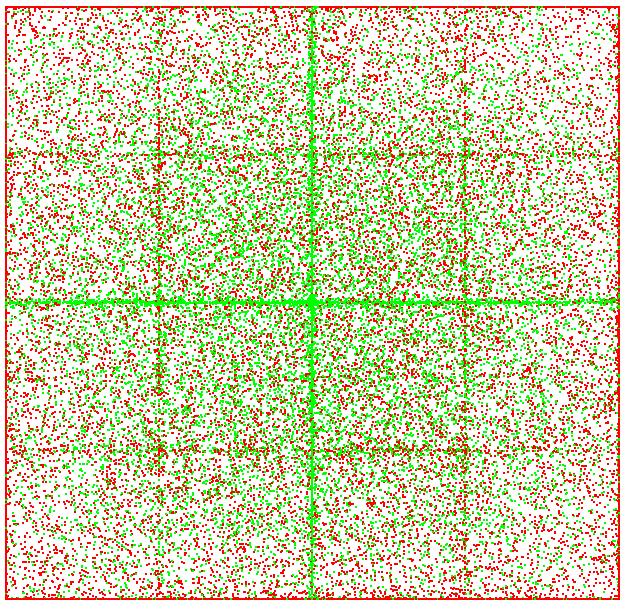
\includegraphics[width=1.0\textwidth, angle=0]{EMERGENT_PATTERN.png}
  	\caption{The emergent pattern used as criteria for qualitative comparison of implementations. Note the big green cross in the center and the smaller red crosses in each sub-sector. World-type is \textit{border} with 100.000 Agents where 25\% are Heroes.}
	\label{fig:EMERGENT_PATTERN}
\end{figure}


\subsection{Problem of RNG}
Have to behave EXACTLY The same: VERY difficult because of differing interfaces e.g. compare java to haskell RNGs.
Solution: create a deterministic RNG generating a number-stream starting from 1 and just counting up. The program should work also in this case, if not, something should be flawed!

Peer told me to implement a RNG-Trace: generate a list of 1000.0000 pre-calculated random-numbers in range of [0..1], store them in a file and read the trace in all implementations. Needs lots of implementation.

\subsection{Run-Time Complexity}
what if the number of agents grows? how does the run-time complexity of the simulation increases? Does it differ from implementation to implementation? The model is O(n) but is this true for the implementation?

\subsection{Simulation-Loops}
There are at least 2 parts to implementing a simulation: 1. implementing the logic of an agent and 2. implementing the iteration/recursion which drives the whole simulation

Classic \\
Yampa \\ TODO: use par to parallelize
Gloss \\
gloss provides means for simple simulation using simulate method. But: are all ABM systems like that?

\subsection{Agent-Representation}
Java: (immutable) Object
Haskell Classic: a struct
Haskell Yampa: a Signal-Function
Gloss: same as haskell classic
Akka: Actors

\subsection{EDSL}
simplify simulation into concise EDSL: distinguish between different kind if sims: continuous/discrete iteration on: fixed set, growing set, shrinking set, dynamic set. 

\section{Conclusion and further research}

So far we only looked at recursive simulation in a simulation with a strictly sequential update-strategy where agents are updated in sequence after each other as defined in TODO: cite my Art-Of-Iteration Paper. We leave the question of how Meta-ABS would apply to the parallel update-strategy and whether it is reasonable to extend it to that strategy or not for further research.

Research Questions
\begin{enumerate}
	\item How does deep regression influence the dynamics of a system? Hypothesis: TODO
	\item How do the dynamics of a system change when using perfect information or learning local information? Hypothesis: TODO
	\item Is a hidden markov model suitable for the local learning? Hypothesis: TODO
	\item How can MetaABS best be implemented? Hypothesis: implementing a MetaABS EDSL in a pure functional language like Haskell, should be best suited due to its inherent recursive, declarative nature, which should allow a direct mapping of features of this paradigm to the specification of the meta-model
\end{enumerate}

Problems
\begin{itemize}
	\item Definition of a recursive, declarative description of the Model.
	\item Perfect information about other agents is not realistic and runs counter to agent-based simulation (especially in social sciences) thus an Agent needs to be able to have local, noisy representations of the other agents.
	\item Local representation of other agents could be captured by Hidden Markov Models: observe what other agents do but have hidden interpretation of their internal state - these internal state-representations can be different between the local and the global version whereas the agent learns to represent the global version as best as possible locally.
	\item Infinite regress is theoretically possible but not on computers, we need to terminate at some point
\end{itemize}

\section{Further Research}
\label{sec:further_research}
We see this paper as an intermediary and necessary step towards dependent types for which we first needed to understand the potential and limitations of a non-dependently typed pure functional approach in Haskell. Dependent types are extremely promising in functional programming as they allow us to express stronger guarantees about the correctness of programs and go as far as allowing to formulate programs and types as constructive proofs which must be total by definition \cite{thompson_type_1991, mckinna_why_2006, altenkirch_pi_2010}.

So far no research using dependent types in agent-based simulation exists at all. In our next paper we want to explore this for the first time and ask more specifically how we can add dependent types to our pure functional approach, which conceptual implications this has for ABS and what we gain from doing so. We plan on using Idris \cite{brady_idris_2013} as the language of choice as it is very close to Haskell with focus on real-world application and running programs as opposed to other languages with dependent types e.g. Agda and Coq which serve primarily as proof assistants.

We hypothesize that dependent types could help ruling out even more classes of bugs at compile time and encode invariants and model specifications on the type level, which implies that we don't need to test them using e.g. property-testing with QuickCheck. This would allow the ABS community to reason about a model directly in code. We think that a promising approach is to follow the work of \cite{brady_correct-by-construction_2010, brady_idris_2011, brady_programming_2013, fowler_dependent_2014, brady_state_2016} in which the authors utilize GADTs to implement an indexed monad which allows to implementation correct-by-construction software.

\begin{itemize}
% NOTE: ran out of space
%	\item Accessing the environment in section \ref{sec:adding_env} involves indexed array access which is always potentially dangerous as the indices have to be checked at run-time. Using dependent types it should be possible to encode the environment dimensions into the types. In combination with suitable data types for coordinates one should be able to ensure already at compile time that access happens only within the bounds of the environment.

	\item In the SIR implementation one could make wrong state-transitions e.g. when an infected agent should recover, nothing prevents one from making the transition back to susceptible. 
	
	Using dependent types it should be possible to encode invariants and state-machines on the type level which can prevent such invalid transitions already at compile time. This would be a huge benefit for ABS because many agent-based models define their agents in terms of state-machines.
	
	\item An infected agent recovers after a given time - the transition of infected to recovered is a timed transition. Nothing prevents us from \textit{never} doing the transition at all. 
	
	With dependent types we should be able to encode the passing of time in the types and guarantee on a type level that an infected agent has to recover after a finite number of time steps.
	
	\item In more sophisticated models agents interact in more complex ways with each other e.g. through message exchange using agent IDs to identify target agents. The existence of an agent is not guaranteed and depends on the simulation time because agents can be created or terminated at any point during simulation. 
	
	Dependent types could be used to implement agent IDs as a proof that an agent with the given id exists \textit{at the current time-step}. This also implies that such a proof cannot be used in the future, which is prevented by the type system as it is not safe to assume that the agent will still exist in the next step.

	\item In our implementation, we terminate the SIR model always after a fixed number of time-steps. We can informally reason that restricting the simulation to a fixed number of time-steps is not necessary because the SIR model \textit{has to} reach a steady state after a finite number of steps. This means that at that point the dynamics won't change any more, thus one can safely terminate the simulation. Informally speaking, the reason for that is that eventually the system will run out of infected agents, which are the drivers of the dynamic. We know that all infected agents will recover after a finite number of time-steps \textit{and} that there is only a finite source for infected agents which is monotonously decreasing. 
	
	Using dependent types it might be possible to encode this in the types, resulting in a total simulation, creating a correspondence between the equilibrium of a simulation and the totality of its implementation. Of course this is only possible for models in which we know about their equilibria a priori or in which we can reason somehow that an equilibrium exists.
\end{itemize}

\newpage

\bibliographystyle{acm}
\bibliography{../../references/phdReferences}

\end{document}